% Todo:
% 
% 
% 
% 
%%%%%%%%%%%%%%%%%%%%%%%%%%%%%%%%%%%%%%%%%%


% コンパイル:
% extractbb img/*.png
% platex soturon.tex
% pbibtex soturon
% platex soturon.tex
% dvipdfmx soturon

\documentclass[12pt]{jreport}

\usepackage[dvipdfmx]{graphicx}
\usepackage{url}
\usepackage{listings, jlisting}
\usepackage{filecontents}

%\usepackage{slashbox}
%\usepackage{amsmath}
%\usepackage{txfonts}

\newcommand{\todayd}{\the\year--\the\month--\the\day}
\newcommand{\argmax}{\mathop{\rm argmax}\limits}
\renewcommand{\bibname}{参考文献}


\title{対戦型パズルゲームにおける機械学習AIと人間の知識を用いたAIの比較}
\date{\today}
%\headtitle{平成28年度 総合情報学科 卒業論文中間発表}
%\affiliation{総合情報学科 メディア情報学コース}
\author{1310163 柴澤弘樹}
%\supervisor{橋山智訓 准教授}

%タイトルページは別作成

\begin{document}

\pagenumbering{roman}
\tableofcontents

\chapter{序論} \label{zyo} \setcounter{section}{0}
\pagenumbering{arabic}
\section{背景}
%遊びとコンピュータゲームの歴史
我々人類は、遊びと共に生きている。ホイジンガは「ホモ・ルーデンス」の中で、遊びが文化よりも古いものであると述べた\cite{homo}。現在遊ばれているコンピュータゲームもまた、遊びの一種といえる。藤田による調査\cite{huzita1,huzita2,huzita3}の中で、コンピュータゲームの一般への普及は、1980年代からであったことが述べられている。

%スマフォによる一般へのゲーム普及、e-sportの市場拡大
現在では、スマートフォンの普及と共にゲームプレイヤーがさらに増えている。ファミ通ゲーム白書2016\cite{famitu}により、スマートフォン・タブレット向けのアプリゲームを含むゲーム市場の拡大が示されている。さらには、eスポーツとして、コンピュータゲームをスポーツのようにプレイヤー及び観客として楽しむ大会も多く開催されてきた。大会やプロプレイヤーにはスポンサーがつき、世界規模の市場となっている\cite{e-sports}。これらの市場は、今後もますますの成長が期待される。

%ネット対戦、AIは対戦相手として不足
%このような背景の下で、遊びとしてのコンピュータゲームはより身近なものになっている。様々なプラットフォームからインターネットを介した協力、対戦プレイが可能となっており、遠く離れたプレイヤー同士で同じゲームをプレイすることも当然のこととなった。それによって、遊び相手として人間が一般的になり、AIを相手に長時間遊ぶゲームは限られたものとなってきている。ゲームAI技術は著しい発展を遂げてきたものの、遊び相手としては未だ向上の余地があるといえる。

%なぜAIである必要があるか? マッチング、練習、環境、対人への抵抗
%インターネットを介した対人プレイにおいては、以下のような問題が挙げられる。
%\begin{itemize}
%\item 対応した環境の必要性
%\item 十分なプレイ人口の必要性
%\item プレイスキルを考慮したマッチング
%\item 気兼ねない相手とはならない
%\item 対人への抵抗感
%\end{itemize}

%環境とは、ゲームのハードウェア、ソフトウェアの両面で整っている必要がある。インターネット環境が整わない場所や、特定のプラットフォームのみでしかプレイできないゲームではオンラインプレイが不可能となる。プレイ人口は、時間や発売からの経過日数などの影響を受ける。一般にゲーム発売後徐々にプレイヤーは減少するが、十分にプレイヤーが揃わなければ、マッチングができない。またプレイスキルのバランスを考慮したマッチメイキングも必要となる。また相手が人間であるため、他プレイヤーを無視した勝手なふるまいが全くできない。ゲームを楽しんだり練習したりするため、あえて無駄な動きや非効率な行為をすることができないのである。また心情的に、他人とゲームをプレイすることを忌避するプレイヤーも一定数いると考えられる。

%以上の問題の通り、遊び相手としての人間が、必ずしも適しているとはいえない場面が存在する。このとき、ゲームAIは一つの解決策となる。そのため、プレイヤーに楽しさを提供する手法を研究し、遊び相手としてのAIを実現することに一定の意義があると考えられる。

%学術研究、コンペティション、強いAI
一方、これまでのコンピュータゲームのAIに関する研究では、人間と対戦する強いAIを目指したものが多かった。IEEE CIG\cite{cig}をはじめとするAIコンペティションや、プロプレイヤーと対戦するAIの開発を通じて、その強さが競われてきた。特に盤上ゲームでは、1997年のDeep Blue、2013のponannza、そして2015年のAlphaGo\cite{alphaGo}が、それぞれプロ棋士に初勝利を収めた。いまやAIは、人間と同等以上の強さをもつようになり、一定の成果が得られたと言われるようになってきている。

%探索アルゴリズム、モンテカルロ法
強いAIを求めるこれまでの研究は、評価の設定と探索アルゴリズムの研究であったという見方ができる。完全情報ゲームの着手に対しどのような評価を与え、計算資源の中でいかに効率よく探索を行うかが問題となってきた。現在までに、着手に評価を与え、最適解を探索する手法が様々提案されている。

その中でAlphGoは、ディープニューラルネットワークによる評価関数の学習、モンテカルロ木探索によってそれらの問題を解決した。ディープラーニングによって、評価関数を事前知識なしに学習でき、従来のAIを上回ることができたことが示された。それまでの研究では、人が設計したルールに基づく評価の設定が主な手法であったため、事前知識の無い学習による評価設定の手法が、大きな成果となった。
この手法によって強いAIの作成は可能となったが、内部でどのような処理が行われているかはブラックボックスとなっている。そのため、学習結果が再利用できないという問題がある。その一方でディープラーニングは汎用性が高く、様々な問題に応用されている\cite{NE, monte}。完全情報ゲームに関しては十分な成果が得られたことから、今後の強さに関する研究は、不完全情報ゲームやGeneral Game Playing(GGP)へ移行してゆくと思われる。

%実際の恩恵、ユーザエクスペリエンスの向上を目的としたAI: miyake, yan_panorama
これまでのゲームAIは、その強さや性能を評価する場として、ゲームを用いていた。現在のAIでは、人間プレイヤーのユーザエクスペリエンスを向上させる域には達していない。強さが十分な領域に達したことで、今後はユーザエクスペリエンスを考慮したAIの研究が活発化してゆくといわれている\cite{miyake_genzai, ikeda}。Yannakakisは今後展開されるべきゲームAI研究の分野を以下の10個に分類した\cite{yan_panorama}。
\begin{enumerate}
\item Non-player character(NPC) behavior learning
\item Search and planning
\item Player modeling
\item Games as AI benchmarks
\item Procedural content generation
\item Computational narrative
\item Believable agents
\item AI-assisted game design
\item General game AI
\item AI in commercial games
\end{enumerate}

1は機械学習によって、ゲームを上手にプレイ出来るふるまいを学習させるものである。2はゲームを探索問題として捉えて、意思決定を行う手法を研究する分野である。3では、人間プレイヤーの知覚や行動をモデル化し、応用することを目指す。4ではAIの性能を確かめ、競うためにゲームを用いる。5はゲームの要素であるマップやステージ構成、アイテムなどを自動生成することを目指している。6では、ゲームのプレイ内容から物語を生成する方法を研究する。7は、AIのプレイ行動などを人間らしくすることが目的である。8では、AI技術を用いてゲームデザイン、すなわちゲーム制作を助けることを目指す。9は特定の種類のゲームに対してではなく、複数のゲームや、ゲームの枠を超えた総合的なAIの確立を研究する。そして10では、学術研究でのゲームAIと切り離されて考えられてきた商業ゲームのAIについて、独自の研究がなされていることを示した。

競争としてのみではなく、ゲームデザイナーやプレイヤーのことを考慮したAI研究がなされていることが分かる。ゲームの遊びや楽しさというユーザエクスペリエンスの側面が、今後ますます注目されてゆくことが予想される。


\section{目的}
%ぷよぷよ:e-sportsの実績、技術レベルの幅広さ、AIがダメダメ、探索問題としての難しさ
本研究では、人を楽しませる相手としてのAIを構成することを目的とする。まず、不完全情報ゲームにおいてAIの強さに関する研究を行い、その後、楽しみについての検討を重ねる。本論文では基礎的検討のためにパズルゲームの「ぷよぷよ」を対象とし、その対戦AIを実装することとした。「ぷよぷよ」は、以下のような特徴をもつ。
\begin{itemize}
\item 長年にわたって親しまれているゲームである
\item 大会やe-sportsでの対戦実績がある
\item プレイヤースキルの幅が非常に広い
\item 対戦用AIの性能が不十分である
\item 不完全情報ゲームであり、探索問題として難しい題材である
\end{itemize}

「ぷよぷよ」は長年にわたって、対戦ゲームとして親しまれてきた。それにも関わらず、未だ強い対戦相手としてのAIは実装ができていない。また不完全情報ゲームであり、探索問題としても課題が残されている。以上の観点から、「ぷよぷよ」のAIが研究対象として意義をもつと考えられる。

様々なコンピュータゲームの多くに不完全情報ゲームがあり、商業用ゲームではこれらのAIが、開示されていないはずの情報を参照することが行われている\cite{yan_panorama}。そのような仕様はプレイヤーに不公平感を与え、楽しさを阻害する可能性がある。このような不正をせずに強いゲームAIを実現することが求められる。

今回は、Yannakakisが提案した10分類のうち、1のNPC behavior learningおよび2のSearch and planningをターゲットとすることになる。まずは強いAIのために、従来のような人が設計し、人の知識を適用したルールベースのAIと、機械学習によって評価関数を学習したAIの双方を実装し、比較を行う。これによって、どちらの手法がより優れているかを確かめ、今後の研究指針とすることが目的である。


%人を楽しませる対戦AI:連鎖、戦術
%連鎖構築が不十分:連鎖数、柔軟性、リアルタイム性

\section{本論文の構成}
本論文の構成は、以下の通りである。第\ref{zyo}章では、研究の背景と目的について述べる。第\ref{puyopuyo}章で、ぷよぷよについて、製品や対戦文化などの背景、ルールと技術的課題について述べる。第\ref{research}章で関連研究として、ゲームAIとゲームの楽しさに関する研究、そしてこれまでのぷよぷよAIを取り上げる。第\ref{dqn}章ではディープラーニングの手法として、「DQN」を用いたぷよぷよのプレイAIの実装を行い、連鎖構築能力と強さを検証する。第\ref{potential}章では従来研究で扱われてきたぷよぷよの連鎖構築アルゴリズム「ポテンシャル最大化法」を検証し、人の手によって設計されたAIの現状と、人の知識を適応する余地について検討する。第\ref{human}章では連鎖ポテンシャル法に人の知識を適用し、ルールベースAIの可能性について示す。最後に第\ref{ketu}章で研究成果と今後の課題を述べ、結びとする。


\chapter{ぷよぷよについて} \label{puyopuyo} \setcounter{section}{0}
「ぷよぷよ」は、落ちものパズルゲームの代表例として、テトリスに並ぶ知名度を誇る。ぷよぷよの代表作である、「ぷよぷよ通」のゲーム画面の様子を図\ref{fig:puyotsu}に示す。「ぷよぷよ」シリーズは、絵柄の可愛らしさ、キャラクターの豊富さ、ルールの単純さから、発売から現代に至るまで広く親しまれている。色のついたブロックを4つ繋げると消える、という単純なルールのため、誰でも楽しむことができるゲームである。その一方で、対戦では連鎖を始めとする様々な戦術による奥深さがあり、コアなプレイヤーも存在して腕を競っている。そのような「ぷよぷよ」について、本章では発売タイトルやルール、対戦の概要やAIの要件について述べる。

\begin{figure}[bt]
  \begin{center}
  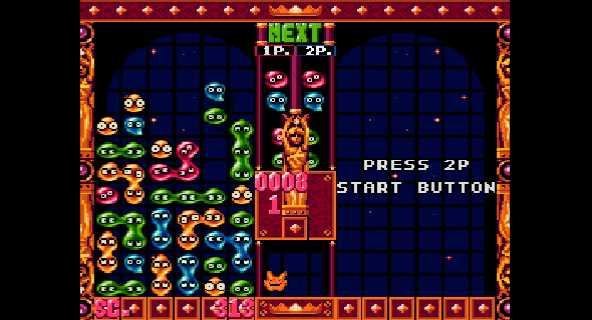
\includegraphics[height=6cm]{img/dqn_toko_5chain.jpg}
  \caption{「ぷよぷよ通」のゲームの様子} \label{fig:puyotsu}
\end{center}
\end{figure}

\section{発売タイトル}
最初の「ぷよぷよ」は、コンパイルより1991年に発売された。当初の「ぷよぷよ」には相殺がなく、1994年の「ぷよぷよ通」によってはじめて導入された。以降のシリーズの基本形はこの「ぷよぷよ通」であるとされ、AC(アーケード)版は現在でも大会で利用される。その後もシリーズは続いたものの売り上げは振るわず、コンパイルは経営破綻に陥った。

2003年の「ぷよぷよフィーバー」以降はセガによってぷよぷよが発売されている。2004年のWindows版「ぷよぷよフィーバー」で、初の公式ネット対戦が可能となった。対戦ルールは「クラシックルール」(実質的な「通」ルール)と「フィーバールール」が搭載されていた。
その後も家庭用ゲーム機や携帯ゲーム機に向けて複数のタイトルが発売されている。2014年には「ぷよぷよ」と同じく落ちものパズルゲームの「テトリス」を組み合わせた、「ぷよぷよテトリス」が発売された。「テトリス」と「ぷよぷよ」の対戦が可能となるなど、異色の作品であった。「ぷよぷよ」のルールは、主に「ぷよぷよ通」に準拠したものとなっている。最新作は2016年発売の「ぷよぷよクロニクル」で、インターネット対戦では「スキルバトル」「ぷよぷよ通」「ぷよぷよフィーバー」の3種類のルールがプレイできる。

その他、「ぷよぷよ!!クエスト」や「なぞぷよ」などの派生作品が、スマートフォン向けアプリなどで発売されている。これらはグラフィックやキャラクター、4つつながると消える点などは踏襲しているものの、対戦要素が無くシステムも異なるため、従来のぷよぷよシリーズとは別のゲームであるといえる。

シリーズ全体を通し、特に対戦において「ぷよぷよ通」が基準となっていることが読み取れる。これまでに様々な新ルール搭載のタイトルが発売されてきたものの、「通」のルールに置き換わるものは未だ現れていない。そこで本稿でも「ぷよぷよ通」のルールに準拠し、以下の「ぷよぷよ」に関する研究を進める。

\section{ルール} \label{rule}
本研究で扱う、「ぷよぷよ通」の基本的なルールと用語について説明する。

%フィールド、ツモ
%ツモ:ペア、ネクスト・ネクネク、4色、自分と相手は同一、
\subsection{フィールドとぷよ} \label{field_puyo}
\begin{figure}[tb]
  \begin{center}
  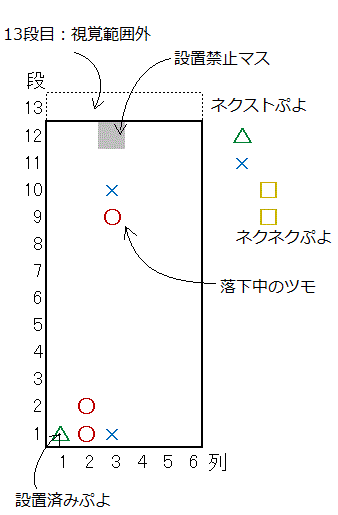
\includegraphics[height=8cm]{img/field.png}
  \caption{ぷよぷよのゲーム画面の概略} \label{fig:field}
\end{center}
\end{figure}

ぷよぷよのゲーム画面の概略図を、図\ref{fig:field}に示す。ぷよぷよのフィールドは、横6列$\times$縦12段が可視範囲である。以下、列数は左から数えたもの、段数は下から数えたものとする。配置するブロックは「ぷよ」と呼ばれる。3列目、12段目のマスにぷよを置くと窒息であり、負け(ばたんきゅ~)となる。また、実際にはフィールドに13段目があり、12段目にぷよがある状態で「回し」という操作技術を用いて、視覚範囲外へぷよを設置できる。13段目のぷよは可視できない状態で繋がったり消えたりすることはなく、12段目以下のぷよを消し、落下させることで連鎖に寄与する。

配石は2つのぷよがペアで現れ、これをツモという。ツモは落下中の物のほかに、次のツモ(ネクストぷよ)と次の次のツモ(ネクネクぷよ)が予め表示される。ぷよは複数の色から成り、対戦では最大4色が標準である。すなわち、4色のぷよが2つずつ現れることから、ツモは全16通りが存在する。回転操作による色の入れ替えを考慮すると、10種類の組み合わせが存在することになる。対戦におけるツモ順は各プレイヤーで同一である。ツモの配色はランダムであり、表示される手数に上限があることから、配石に関する情報の不完全性が認められる。

ツモは3列目の13段目と12段目に現れ、自然に落下してゆく。落下中のツモは左右移動と左右回転ができるため、すでに埋まっていない限りは任意の列、あるいはそれと隣り合った列に配置できる。ぷよの設置の際は、下段に空白を認めない。下に空洞がある場合、それより上のぷよは全て下に落下する。よって、段差がある隣り合った2列に対しツモを横向きに置いた場合、片方のぷよが落下する。これを「ちぎる」という(図\ref{fig:tigiri}参照)。ツモの配置方法の選択は、異なる色の場合22通り、同色(ゾロ)の場合11通りとなる。
\begin{figure}[tb]
  \begin{center}
  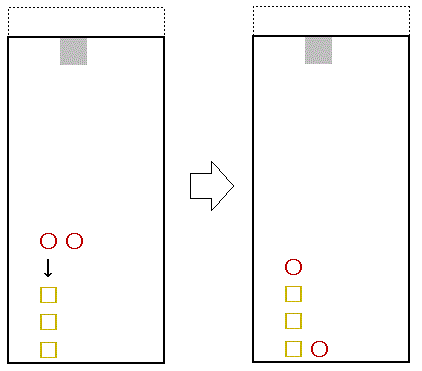
\includegraphics[height=5cm]{img/tigiri.png}
  \caption{「ちぎり」の発生の様子} \label{fig:tigiri}
\end{center}
\end{figure}

%消去、連鎖
\subsection{ぷよの消去と連鎖} \label{del_chain}
置かれた色ぷよは、上下左右に隣接したマスの同色ぷよと連結する。ここで色ぷよとは、後述の「おじゃまぷよ」ではない、ツモによって配されたぷよのことである。接続数が4以上となったぷよは、その時点ですべて消える。ぷよが消えたマスは空白となるが、その上部に別のぷよが存在する場合には、その落下により空白は埋められる。

\begin{figure}[tb]
  \begin{center}
  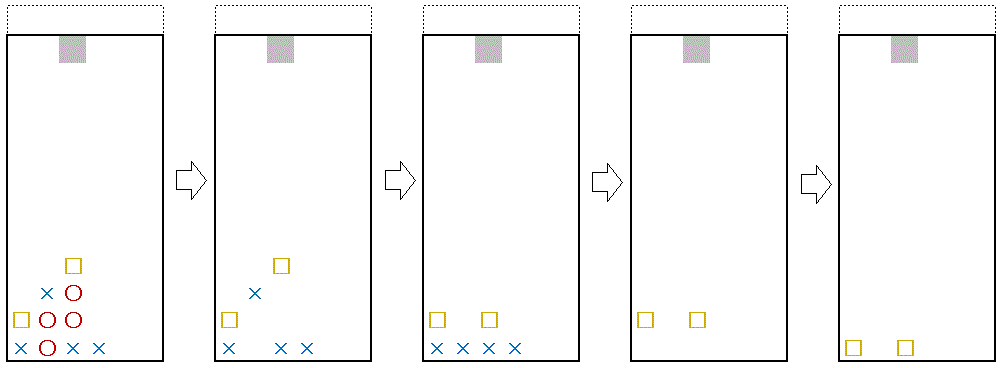
\includegraphics[height=5cm]{img/rensa.png}
  \caption{「連鎖」の発生の様子} \label{fig:rensa}
\end{center}
\end{figure}

ぷよが消えた後の落下により、さらに4つ以上接続されたぷよが現れた場合には、連続でぷよの消去が発生する(図\ref{fig:rensa}参照)。これを連鎖という。連続での消去が$n$回発生した際には$n$連鎖となる。ぷよが消えるために最低4つを必要とし、フィールドは全78マスであるから、最大連鎖数は19連鎖である。また、連鎖を発動させるためにぷよを消去することを、「発火」という。

発火時には3列目12段目にもぷよを設置することができ、即座にはゲームオーバーとならない。ぷよの消去および連鎖の発生中には、新たなツモは発生せず、プレイヤーは操作ができない。連鎖がすべて終了した後に、操作可能となる。この時、3列目12段目にぷよが残っていると、その時点でゲームオーバーとなる。

%予告ぷよ、相殺、降るタイミング
%スコア
\subsection{スコアとおじゃまぷよ} \label{score_ojama}
ゲーム中には各プレイヤーのスコアが計算される。スコアは下キーによるぷよの落下操作時と、ぷよの消去および連鎖時、全消し時に増加し、1ゲーム中に減少することはない。落下操作時には、1マスにつき1点が加算される。全消しの際には2100点が加算される。$n$連鎖におけるスコアは、式\ref{fo:score}で算出できる。

\begin{eqnarray} \label{fo:score}
score & = & \sum_{i=1}^{n}(score_{i}) \nonumber \\
& = & \sum_{i=1}^{n}(delPuyo_{i} \times 10 \times bonus_{i})
\end{eqnarray}
ここで、$score$は発動した連鎖の合計スコア、$score_{i}$は$i$連鎖目のみのスコア、$delPuyo_{i}$は$i$連鎖目で消えたぷよの数、$bonus_{i}$は$i$連鎖目でのボーナス係数を表す。

ボーナスは、以下の3つのボーナスの総和で表される。
\begin{itemize}
\item 多色ボーナス:同時に消した色の数によるボーナス
\item 連結ボーナス:消したぷよの接続数によるボーナス
\item 連鎖ボーナス:連鎖数によるボーナス
\end{itemize}
それぞれのボーナス値を、表\ref{tab:color_bonus}、表\ref{tab:connect_bonus}、表\ref{tab:chain_bonus}に示す。ただし、ボーナスの総和が0の時には、値を1とする。

\begin{table}[tb]
\begin{center}
\caption{多色ボーナス} \label{tab:color_bonus}
\begin{tabular}{|l|r|r|r|r|} \hline
色数 & 1 & 2 & 3 & 4\\ \hline
ボーナス & 0 & 6 & 12 & 24\\ \hline
\end{tabular}
\end{center}
\end{table}

\begin{table}[tb]
\begin{center}
\caption{連結ボーナス} \label{tab:connect_bonus}
\begin{tabular}{|l|r|r|r|r|r|r|r|r|} \hline
連結数 & 4 & 5 & 6 & 7 & 8 & 9 & 10 & 11以上\\ \hline
ボーナス & 0 & 2 & 3 & 4 & 5 & 6 & 7 & 10\\ \hline
\end{tabular}
\end{center}
\end{table}

\begin{table}[tb]
\begin{center}
\caption{連鎖ボーナス} \label{tab:chain_bonus}
\begin{tabular}{|l|r|r|r|r|r|r|r|r|r|r|} \hline
連鎖数 & 1 & 2 & 3 & 4 & 5 & 6 & 7 & 8 & 9 & 10\\ \hline
ボーナス & 0 & 8 & 16 & 32 & 64 & 96 & 128 & 160 & 192 & 224\\ \hline \hline
連鎖数 & 11 & 12 & 13 & 14 & 15 & 16 & 17 & 18 & 19 & -\\ \hline
ボーナス & 256 & 288 & 320 & 352 & 384 & 416 & 448 & 480 & 512 & -\\ \hline
\end{tabular}
\end{center}
\end{table}

対戦では、算出されたスコアに応じて、対戦相手におじゃまぷよが降る。スコア70点がおじゃまぷよ1つに相当する。70点以下は切り捨てられ、次回に持ち越される。対象となるスコアは、これまでにおじゃまぷよに換算されていないすべてのスコアである。つまり、落下操作や全消しで加算されたスコアは、次のぷよの消去時におじゃまぷよの換算に使われる。

おじゃまぷよは連鎖終了後、相手が落下中のツモを設置した時点(相手が次のツモを引く前)で降る。おじゃまぷよの落下列は都度ランダムに選ばれる。ただし一度に複数のおじゃまぷよが落ちる際には、偏りが少なくなるように落下列が選ばれる。例えば6個以下のおじゃまぷよが2段以上で降ることはなく、おじゃまぷよ6個はすべての列に1つずつ降る。なお、一度に降るおじゃまぷよの数は30個(5段)が上限であり、一度おじゃまぷよが降ると次の一手が配される。上限を超えておじゃまぷよが存在する場合、1手のツモを置いたのちに再度降ってくることとなる。

自分のフィールドにおじゃまぷよが降るまでには、相手の連鎖発火から連鎖が終了し、さらに自分が1手を置くまでの猶予がある。相手からおじゃまぷよが送られている間に自分の連鎖を発火すると、おじゃまぷよの相殺ができる。相殺の後に得点の高かったプレイヤーが、相手にスコアの差分だけおじゃまぷよを降らすことができる。相殺の途中で相手の連鎖が終了しており、かつ相殺し切れなかった場合には、自分の連鎖終了後即座におじゃまぷよが降って来る。
%タイムテーブル

\section{ぷよぷよの対戦}
\subsection{対戦文化と大会}
%95年:全日本ぷよマスターズ大会、ばよえ~んツアー
ぷよぷよの対戦は、ゲームの発売以降長い間にわたって続いてきた。公式大会の歴史は1995年にまでさかのぼることができ、コンパイル主催で「全日本ぷよマスターズ大会」や「ばよえ~んツアー」などが大々的に行われていた。

%100本先取
公式大会以外にも、有志によるゲームセンターやインターネット上での大会は数多く行われてきた。特に上位プレイヤーは、ゲームセンターのAC版「ぷよぷよ通」で強さを競い、全日本一位の座を目指した。試合形式は100本先取戦とされ、時として200試合近くに及ぶ対戦によって勝敗がつけられた。
試合は非公式であったものの、十分に試合回数を重ねることで、偶然性を排した強者のランキングがコミュニティの中で共有されていた。

%対戦文化:大会、e-sports
近年では、eスポーツ人気の高まりに伴い、ぷよぷよの大会にスポンサーがついたり、上位プレイヤーがテレビ番組に出演する機会が増えている。2016年の主な大会では、セガ公式「ぷよぷよ」最強プレイヤー決定戦\cite{sega}、第5回アーケード版ぷよぷよ通S級リーグ\cite{Skyuu}、A級リーグ\cite{Akyuu}、統一王座戦\cite{touituouza}、Red Bull 5G 2016\cite{5g}などが開催された。このように、ぷよぷよの発売以降現在でも、対戦ゲームとしての人気は高い。実用のプレイAIを実装するにあたっては、対戦を念頭に置くことが重要である。

%AIの到達点として、念頭におくべきこと
\subsection{対戦の基本的戦術} \label{senzyutu}
ぷよぷよは相殺のシステムにより、基本的に高い威力の連鎖を保持するプレイヤーが有利となる(\ref{score_ojama}参照)。お互いの連鎖を同時に発火した場合、スコアの高い連鎖が勝ち、一方的におじゃまぷよを送れるためである。連鎖の威力を上げるためには、同時に消すぷよの数や色の数を増やす、連鎖数を増やすといった方法がある。そのように連鎖を組むためには、ぷよを消さずにフィールドに積み上げる必要性がある。以下で、主な戦術を説明する。
\\[.5em]

%小連鎖によるつぶし
1.つぶし\\
フィールドの多くがぷよで埋まっている状態では、少ないおじゃまぷよで残りのフィールドが埋まるために負けやすくなる。つまり、大連鎖を保持するプレイヤーを、小連鎖で倒すことが可能である。倒すまでには至らない場合でも、相手が連鎖を発火できない程度におじゃまぷよを送り、埋めてしまう(つぶし)ことが可能である。このように、単純に大連鎖のみの勝負とはならない奥深さがある。
\\[.5em]

%先打ち有利=>発火催促
2.伸ばし\\
さらに、片方のプレイヤーのみが大連鎖を発火した場面を考える。発火したプレイヤーの連鎖が進んでいる間も、もう片方のプレイヤーは操作が可能である。連鎖の終了までおじゃまぷよは降らないので、複数のツモを使って連鎖をさらに増やすことができる(伸ばし)。相手の連鎖が終了する前に後から伸ばした連鎖を発火すると、相手の連鎖を相殺し、おじゃまぷよを送り返すことすら可能である。このように、最初の発火時点で両者の連鎖威力が同等あるいは不利だったとしても、そのあとで状況を崩して有利にすることが可能である(後打ち有利)。
\\[.5em]

%催促合戦、凝視、組み換え(打つタイミング)
3. 催促\\
大連鎖を先に発火させるべく、相手の発火を促す戦術が成立する(催促)。大連鎖とは別に小連鎖を用意し、そちらを使って相手の発火を催促する戦術である。相殺できなければ潰されてしまい、発火しても不利な状況に陥る。このため、相手の小連鎖に対応するための小連鎖を、自分もまた用意する必要が出てくる。相手の状況を見て(凝視)、自分の連鎖を組む技術が重要になった。

以上で述べた通り、ぷよぷよの対戦にあたっては、連鎖数や威力だけでは語れない駆け引きが生じる。ここで述べた前提を基にして、様々な戦術や連鎖がこれまでに生まれてきた。これらを活用した強いAIを実装することもまた、ぷよぷよAIの重要な課題である。しかし、本稿ではそれを今後の課題とし、まずは大連鎖の構築に着目する。


\section{連鎖構築}
%対戦における実用的な連鎖とは何か? %なぜ連鎖数、柔軟性、リアルタイム性が必要か?
対戦において連鎖は、相手への攻撃手段でもあり、相手からの攻撃に対する防御手段でもある。そのため、連鎖を構築する能力は基本的かつ重要なものとなる。実戦の上で必要となる連鎖構築能力には、連鎖数、柔軟性、リアルタイム性が求められると考える。その内容を以下で説明する。

%連鎖数:フィールドの限界と効率
\subsection{連鎖の威力と連鎖数}
%スコア
連鎖を構築する目的の大部分が、大きなスコアを得るためである。なぜなら、スコアこそが相手に送れるおじゃまぷよの量を決定づけるからである。\ref{score_ojama}で述べた内容から、スコアを大きくするためには、ぷよの消える数や色を増やし、連鎖数を増やすことが有効であると分かる。しかし、フィールドに設置できるぷよの数には限りがあることに注意を要する。すなわち、フィールドを最大限効率よく使うために、同時消しの数をより増やすか、連鎖数をより増やすかを考えなければならない。

\begin{figure}[tb]
  \begin{center}
  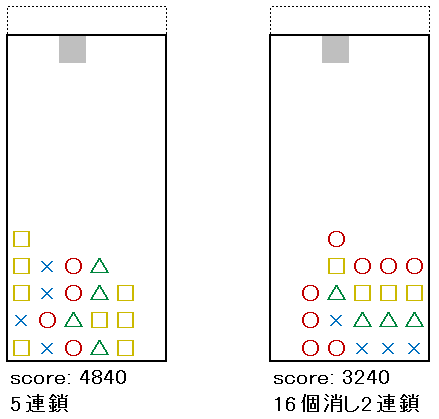
\includegraphics[height=6cm]{img/chain_score.png}
  \caption{連鎖数とスコア} \label{fig:chain_score}
\end{center}
\end{figure}

例えば、20個のぷよを全て消す場合を考える。4個消し5連鎖が合計4840点になるのに対し、2連鎖同時消し(1連鎖目で4個、2連鎖目で4色16個同時消し)では3240点となる(図\ref{fig:chain_score}参照)。つまり、同じぷよの数であれば、同時消しの数を増やすよりも、連鎖数を増やした方が、スコアが高くなる。これは連鎖ボーナス(表\ref{tab:chain_bonus})の上昇幅が大きく、さらに連鎖ごとに繰り返し点数が加算されることに起因する。よって限られたぷよ数で威力の高い連鎖を構築するためには、同時消しの数を減らし、連鎖数の効率を上げることが重要である。

%飽和連鎖量 %おじゃま、同時消し、形
組んでいる連鎖に同時消しの数が多かったり、フィールドにおじゃまぷよが存在していたりすると、必然的に連鎖数の上限が減ってしまう。このような観点から連鎖の効率を考える時、「飽和連鎖量」という概念を用いる。これは、そのまま最大まで連鎖を伸ばしたとき、最終的な威力がどれほどとなるかを示す量である。上級者は経験的に、フィールドの状態からあと何連鎖伸ばすことができ、最終的にどれほどの連鎖威力になるかを判断できる。それを「飽和連鎖量」と呼ぶ。現在保持している連鎖の量だけではなく、将来的にどれほど連鎖数を向上させることが可能かを考えることもまた、重要な能力である。そのような先読みによって、連鎖を完成させることよりもさらに伸ばすための布石を打つことを優先するような工夫ができ、飽和連鎖量を向上させることができる。

%柔軟性:ツモに合わせて完成形を変える %定型、不定形 %途中消し %合体、キーぷよ
\subsection{連鎖の柔軟性}
連鎖は、大きく定型連鎖と不定形連鎖に分けることができる。定型は、決まった連鎖形と名称が知られたものを指し、不定形は定型で無い連鎖を指す。それぞれの連鎖の例を、図\ref{fig:teikei}と図\ref{fig:huteikei}に示す。ぷよぷよでは配されるツモがランダムに決定されるため、それに合わせて連鎖を組む必要がある。定型連鎖では最終形に合わせてツモを配置してゆき、不定形連鎖ではツモに合わせて最終形を変えてゆく。どちらにしても、ツモに合わせて柔軟に配置を決定する必要がある。

\begin{figure}[tbp]
  \begin{center}
  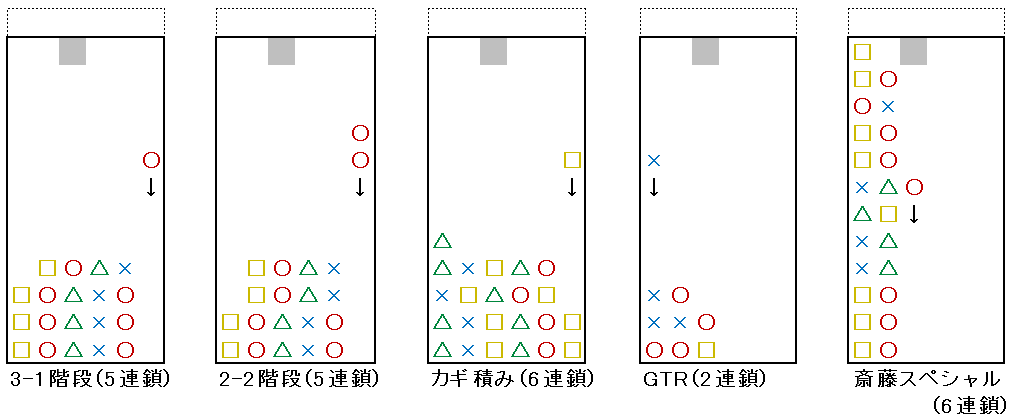
\includegraphics[height=5cm]{img/teikei.png}
  \caption{定型連鎖の例} \label{fig:teikei}
\end{center}
\end{figure}

\begin{figure}[tbp]
  \begin{center}
  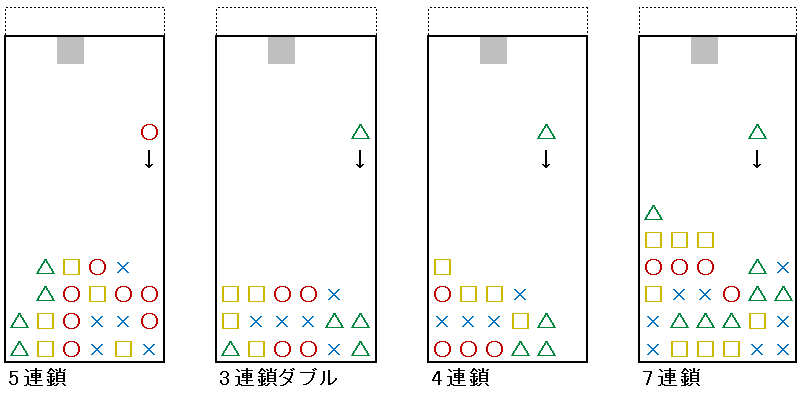
\includegraphics[height=5cm]{img/huteikei.png}
  \caption{不定形連鎖の例} \label{fig:huteikei}
\end{center}
\end{figure}

%定型:色の可換性、おけない、混ぜ定型、途中けし
定型連鎖は完成形が定まってはいるものの、実際に組む時のぷよの配置が、固定化されたものであるとはいいがたい。まず、色の組み合わせに関して厳密に定めることが非現実である。例として3-1階段5連鎖を挙げると、図\ref{fig:kaidan5}に示したものは全て同じ形といえる。このように、同じ連鎖であってもその色の組み合わせは複数あり、完成形をただ一つに定めることができない。そして色の組み合わせは、ツモの落下順によって定まってゆくものである。一見して同じ形を組む場合であっても、ツモに応じた色の配置の変更が必要である。

\begin{figure}[tbp]
  \begin{center}
  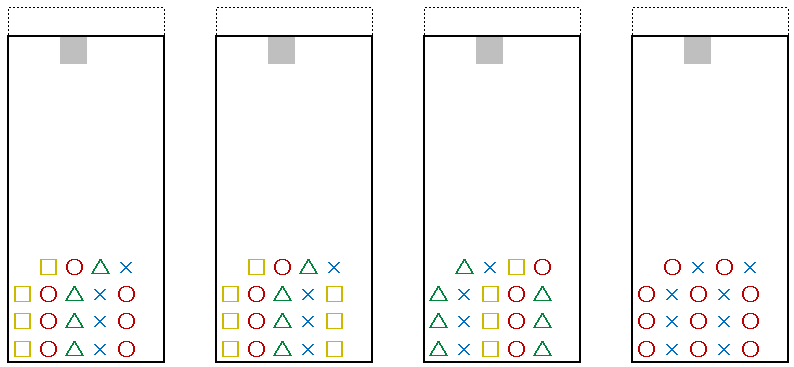
\includegraphics[height=5cm]{img/kaidan5.png}
  \caption{色違いで同形の階段5連鎖} \label{fig:kaidan5}
\end{center}
\end{figure}


\begin{figure}[tbp]
  \begin{center}
  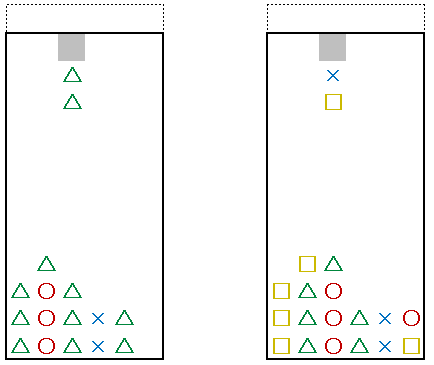
\includegraphics[height=5cm]{img/kaidan_ng.png}
  \caption{3-1階段でツモの置き場が無い例} \label{fig:kaidan_ng}
\end{center}
\end{figure}

\begin{figure}[tbp]
  \begin{center}
  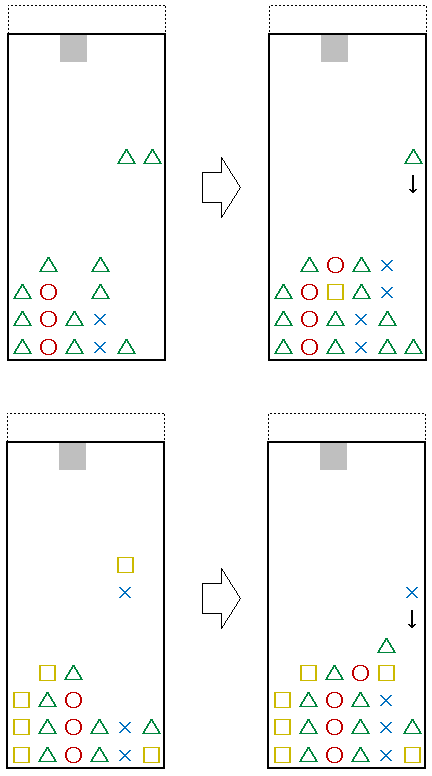
\includegraphics[height=10cm]{img/kaidan_ok.png}
  \caption{工夫した階段連鎖と完成形} \label{fig:kaidan_ok}
\end{center}
\end{figure}

\begin{figure}[tbp]
  \begin{center}
  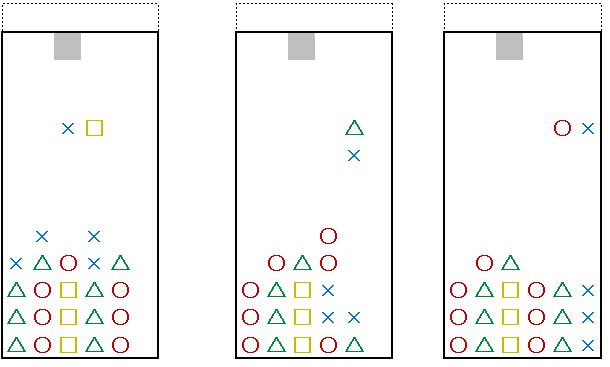
\includegraphics[height=5cm]{img/teikei_del.png}
  \caption{余分なぷよの消去による整地の例} \label{fig:teikei_del}
\end{center}
\end{figure}

\begin{figure}[tbp]
  \begin{center}
  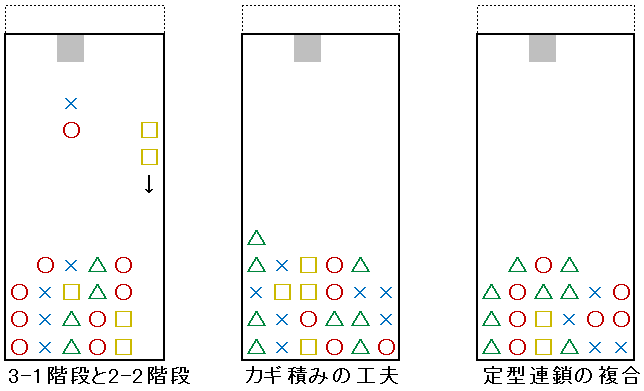
\includegraphics[height=5cm]{img/teikei_combi.png}
  \caption{定型連鎖の改変と組み合わせの例} \label{fig:teikei_combi}
\end{center}
\end{figure}

その上、配置を固定化してしまうと、必ずしもツモを活かせないという欠点が表出する。図\ref{fig:kaidan_ng}で示したような例では、決められた連鎖形にするためにはツモを消すか捨てるかしかできない。しかし同じような場面でも、わずかに形を変えることで図\ref{fig:kaidan_ok}のようにツモを有効活用できる。たとえ定型連鎖であっても、ある程度形を変えられるような柔軟性を持たすことが有効である。ツモに合わせてぷよを配置する柔軟性があって初めて、余分なぷよを消して形を整えたり(図\ref{fig:teikei_del})、定型連鎖をわずかに改変したり(図\ref{fig:teikei_combi})することが可能となる。このような配置の柔軟性をさらに顕著にしたものが、不定形連鎖である。


ツモを有効に活用するためには、配色に合わせて柔軟に形を選択し、ぷよを配置する能力が重要である。特に対戦では、相手からおじゃまぷよが送られてきた場合に、定型連鎖をそのまま維持することが困難となる。さらに相手に合わせた連鎖の用意などを見据えた場合、完成形を定めておくことは困難である。対戦で不定形連鎖が好まれるのは、ツモにあわせて連鎖形を変化させる柔軟性が大きな利点となるためである。


%リアルタイム性:早さによる有利・不利 %ちぎり、連鎖の速度(同時消しの強さ)
\subsection{リアルタイム性}
これまでに、連鎖を組む能力としてぷよの置き方に着目してきた。もう一つの重要な能力が、早さである。この早さには2種類があり、連鎖を組む早さと、連鎖自体の早さが考えられる。

連鎖を組む早さが勝負に影響することは明らかである。同じ威力の連鎖を組めるが、その早さが異なる2プレイヤーの対戦を考える。この場合、片方のプレイヤーが最大連鎖に到達した時点で、もう片方のプレイヤーは相手に劣る威力の連鎖しか保有できていない。当然、連鎖の打ち合いでは速度の遅いプレイヤーが負ける可能性の方が高くなる。威力のポテンシャルが同じでも、リアルタイムに進むゲームであるから、ある時点での保有連鎖量が異なることで有利不利が生じることとなる。

ただし、\ref{senzyutu}で述べた通りに、後から連鎖を打つプレイヤーはさらに連鎖を伸ばす余地がある。相手の連鎖が終了するまでの時間、十分な速度で連鎖を組むことができれば、逆に有利な状況に立てる可能性がある。このように、連鎖を組む速度に応じてリアルタイムに戦況が変化する。早くツモをさばけるプレイヤーの方が、連鎖を増やすことや相手を妨害することにより多くのリソースを費やすことができるため、有利となる。

%連鎖を組む速度を向上させるためには、意思決定の高速化、操作の高速化、ちぎりを少なくするなどの方法がある。段差のある2列に対しぷよを横向きに設置すると、ぷよがちぎれて落下する。ちぎりによる落下速度は下キーの操作による移動よりも遅いため、頻繁に行うとタイムロスにつながる。

また連鎖数が増えると、アニメーションの描画が繰り返されるために発火から連鎖終了までの時間が長くなる。相手に対し即座におじゃまぷよを送りたい場合などでは、連鎖数を少なくする方が有効である。威力を犠牲にしてでも、同時消しや連鎖数の削減により機を逃さずに攻撃すべき局面が存在する。逆に相手が短時間の連鎖を仕掛けてきている時にも、将来的な連鎖数より現時点での短期的な連鎖の完成を目指すべきである。

連鎖構築能力としてのリアルタイム性には、連鎖を構築する早さを高めること、現時点と将来の盤面状況を判断して連鎖を組みかえることが求められる。対戦ではリアルタイム性が高いことを念頭に置き、時間の制約を意識することが肝要である。

\section{ぷよぷよのAI実装における課題}
対戦型の「ぷよぷよ」のプレイでは、連鎖構築や戦術が重要となる。上級者のプレイでは、十分な威力の連鎖を保持しつつ、相手を妨害したり、相手の妨害を阻止したりする戦術が用いられている。現状のAIでは、どちらも不十分であり、十分な強さを得られていない。この解決のためにはまず、より基本的な行為である、連鎖構築を満足に行えなければならない。対戦中での連鎖構築は、連鎖数、柔軟性、リアルタイム性の3点を満足することが大切であると考えられる。本研究では、この3点を満たす連鎖構築アルゴリズムを実現することを目指す。

%解決すべき課題%難しさ、技術的課題:
%・スコア増加の長期的視点(NG:1手で消去, OK:3手で+1連鎖)
%・ランダム性とおじゃまによる先読みの難しさ
%・色の可換性、ツモ順によるパターン化の難しさ
%・累乗オーダでの計算量
%・リアルタイムの制約
「ぷよぷよ」の連鎖構築AIの実装にあたり、技術的課題は以下に挙げられる。
\begin{itemize}
\item 長期的視点に基づく探索
\item 不完全情報と妨害による先読みの難しさ
\item 完成形のパターン化の難しさ
\item 計算量の膨大さとリアルタイムの制約
\end{itemize}

大きな連鎖数を確保するためには、長期的視点に基づいてぷよの配置を決定する必要がある。同じ一手であっても、すぐに連鎖の威力を補強できる手よりも、数手先で連鎖数を増やすための布石とする手の方が有効である。このために先読みが必要になるが、配される手がランダムであること、リアルタイムに相手からの妨害があることを考慮すると、その可能性が膨大になる。このような情報の不完全性から、連鎖の完成形をあらかじめ想定しておくことが大きな手間となる。配された手から完成形を組みかえるような、柔軟性ある連鎖構築が望ましいのはそのためである。最後に、ぷよは操作をしなくとも自由落下するため、配置の決定に時間的制約がある。以上のような課題を解決する手法の実装により、AIの強さを調べることとする。

\chapter{関連研究} \label{research} \setcounter{section}{0}
\section{DQN}
これまでに多くのゲームAI研究がなされてきた。近年は、特定のゲームに関する強さを追求することに一旦の区切りをつけ、様々な応用へと挑戦が進んでいる\cite{yan_panorama, adaptive}。

2015年には、DQN(Deep Q-Network )によるAIがAtari 2600のゲーム49種類の学習を行った\cite{DQN}。その結果、43のゲームで従来研究を上回り、29のゲームでプロの人間プレイヤーと同等以上の性能を示した。この手法では、ゲームの事前知識なしに学習を行い始め、最終的にゲームのプレイ操作を学習するまでに至った。

DQNは、ディープラーニングとQ学習を組み合わせた手法である。それぞれの手法について、以下に簡単に説明する。

\subsection{ディープラーニング}
ディープラーニングは、人間の脳神経回路網をモデルとしたニューラルネットワークを用いた学習モデルである。

ニューラルネットワークでは、複数のニューロン同士を接続し、入出力のネットワークを構成する(図\ref{fig:NN_model}, \ref{fig:NN_InOut})。1つのニューロンには、接続された複数のニューロンからの信号が入力される。その入力を非線形関数で処理し、ニューロンの出力とする。その出力はまた別のニューロンへと入力される。このように、接続を介してニューロン同士で信号をやり取りするのがニューラルネットワークのモデルである。

またそれぞれの接続には結合荷重が設定されており、入出力に影響する。この結合荷重をパラメータとして学習し、最適化を行うのがニューラルネットの学習である。学習には逆誤差伝搬法を用いることが一般的である。逆誤差伝搬法では、出力値の誤差をネットワークへと逆方向に伝搬させ、勾配法により目的関数の誤差を小さくするように結合荷重の値を更新する。

ニューラルネットワークの中でも、ニューロン同士の接続が片方向であり、入力から出力までの信号の流れが定まっているものを順伝搬型という。特に入力層、中間層、出力層のように層を定め、中間層が多数あるネットワークを、ディープニューラルネットワークという。ディープラーニングではディープニューラルネットワークを用いて、入出力のサンプルから任意のモデルを学習できる。ただし、学習結果は結合荷重により分散して記録されるため、必ずしも意味を持つものとは限らない。その解釈は、一般には困難である。

\begin{figure}[tb]
  \begin{center}
  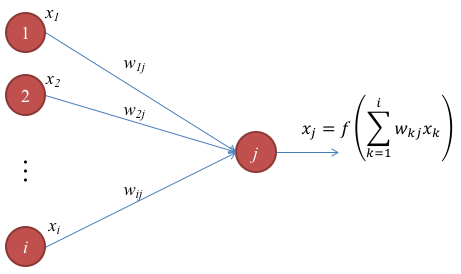
\includegraphics[height=5cm]{img/NN_model.png}
  \caption{ニューラルネットワークの例} \label{fig:NN_model}
\end{center}
\end{figure}

\begin{figure}[tb]
  \begin{center}
  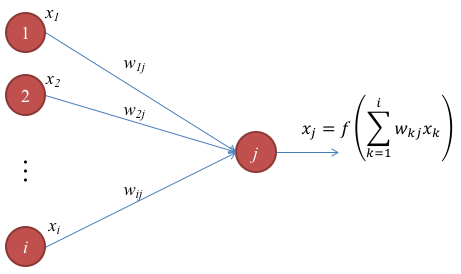
\includegraphics[height=5cm]{img/NN_InOut.png}
  \caption{ニューラルネットワークの入出力} \label{fig:NN_InOut}
\end{center}
\end{figure}

\subsection{Q学習}
Q学習は、行動と環境に伴う報酬によって意思決定を学習する、強化学習の一種である。強化学習では、環境と行動によるモデルを用いる。ある環境$s_{t}$で行動$a$をとると、環境が$s_{t+1}$へと変化をする。この変化による報酬$R_{t+1}$を定め、その後の報酬の期待値である行動価値を最大化する最適戦略を学習する手法である。Q学習では、行動価値をQ関数によって定める。

学習前の時点では、正確な行動価値、すなわちQ($s_t$, $a_t$)は分かっていない。ここで、$s_t$は時点$t$での環境、$a_t$は時点$t$での行動を表す。そこで、始めは各々の$s$、$a$におけるQ($s$, $a$)をランダムに定めた後、以下の式でQ関数の更新を行う。
\begin{eqnarray}
  Q(s_{t}, a_{t}) = Q(s_t, a_t) + \alpha (R_{t+1} + \gamma \max_a Q(s_{t+1}, a) - Q(s_t, a_t)) \nonumber\\
\end{eqnarray}
ここで、$R_{t+1}$は環境$s_t$で行動$a_t$をとったことにより$s_{t+1}$で得られた報酬、$\alpha$は学習係数、$\gamma$は割引き係数を表す。二つの係数は、それぞれ0から1の範囲の実数である。この式は、次の状態における行動価値から、現在の状態での行動価値を更新するものである。

ある状態$s_t$でとるべき行動$a$は、
\[
a = \argmax_a Q(s_t, a)
\]
により定まる。学習が進むにつれてQ関数は実態に近づいてゆく。環境、行動と報酬を定義しておけば、試行を繰り返すことで事前知識無しに最適戦略が定まる。

\subsection{DQN}
DQNは、Q学習におけるQ関数を、ディープニューラルネットワークで表現する手法である。ある時刻$t$におけるゲームの状態$s_t$を入力とするディープニューラルネットワークを用いて、行動$a$に対する評価値(Q値)を出力として得る。ニューラルネットワークのパラメータ$\theta$は、以下の式で更新する。
\begin{eqnarray}
\theta_{t+1}(s_t, a_t) = \theta_t + \alpha (R_{t+1} + \gamma \max_a Q_t(s_{t+1}, a; \theta_t) - Q_t(s_t, a_t; \theta_t))\nabla_\theta Q_t(s_t, a_t; \theta_t) \nonumber\\
\end{eqnarray}
ここで、$a_t$は$t$でとった行動、$R_{t+1}$は$s_t$および$a_t$によって得られた報酬、$\alpha$は学習係数、$\gamma$は割引係数を表す。

DQNを使うための環境の実装には、Atari 2600の環境であるALE(Arcade Learning Environment)\cite{ALE}の他、スーパーファミコン用の環境であるRLE(Retro Learning Environment)\cite{RLE}が存在している。Bhonkerらは5つのスーパーファミコンゲームにおけるDQNの性能を報告している\cite{RLE}。

%ぷよぷよとの関係
%パックマンは偶然による得点の取得が困難?
DQNは事前知識を持たないため、様々なゲームに応用できる汎用性が示されている。ただし、学習の開始時点では操作がランダムとなるため、報酬を偶然的に得ることができないパックマンのようなゲームでは、十分な性能を示せないことが課題となっている。また、ディープニューラルネットワークによる学習のため、学習した知識はブラックボックスとなり、その解析のためにはさらなる技術が必要になる。これらのデメリットにもかかわらず、事前知識を必要とせず、繰り返しのゲームプレイからゲームに関する知識を得られるこの手法は、強力なものである。

現状では、ぷよぷよのようなパズルゲームに対するDQNの研究は未だなされていない。ぷよぷよは4つ以上のぷよをつなげることで得点を得られるが、これはランダムなゲーム行動の中でも起き得る現象である。同様に、学習の中で連鎖が起きる可能性も十分にありうる。そのため、DQNによりぷよぷよの連鎖構築知識が得られるかを確かめることとした。

\section{ゲームと楽しさ}
「楽しさ」とは何か、という問いは分野を問わず、難しい問題である。人は様々な場面で楽しさを感じるが、それが本質的にどういったものかを明確に示すことは難しい。

Csicszentmihalyi\cite{csikszentmihalyi}は、楽しさを「フロー理論」によってモデル化した。フロー理論では楽しさを、物事に没入したフロー状態として捉える。フロー状態は、人のスキルと課題の挑戦度がちょうど良いバランスとなった場合にのみ起きると主張される(図\ref{fig:flow}参照)。スキルに対して課題が簡単過ぎれば退屈であり、課題が難し過ぎれば不安となって没入を妨げる。フロー状態は、様々なゲームやスポーツ、さらには日常生活においても起こりうるものである。

\begin{figure}[tb]
  \begin{center}
  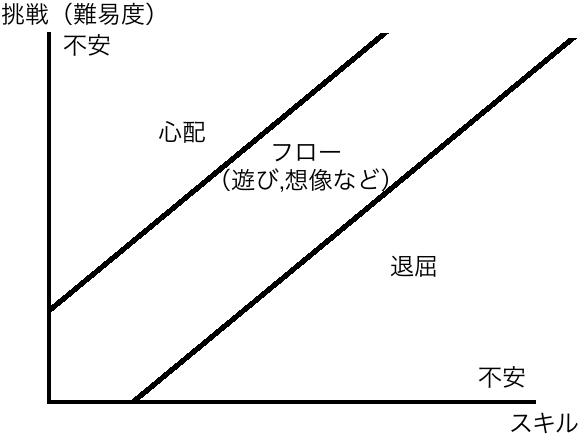
\includegraphics[height=5cm]{img/flow_theory.png}
  \caption{フロー理論の概略図} \label{fig:flow}
\end{center}
\end{figure}

Malone\cite{malone}は、コンピュータゲームの楽しさに着目し、「挑戦」「好奇心」「ファンタジー」が重要であると主張した。挑戦はCsicszentmihalyiと同様であり、それに加えて予測不可能性やランダム性としての好奇心と、表現やデザインとしてのファンタジーを要素に挙げた。Maloneの観点からは、同じレベルの挑戦にも、プレイヤーの知識に応じた質的な違いが生じうることを考慮できる。

これらのモデルは様々な娯楽やゲームに適応できる汎用的なものである。そのため、実際にはどのようなゲーム要素が楽しさの因子となるかを、具体化することが求められる。山下ら\cite{tanosisa}はアンケート調査によってゲームの楽しさの因子を分析した。「ゲーム本来の楽しさ」という因子には「挑戦的な」「好奇心を駆り立てる」などが含まれ、Maloneの主張を裏付けた。さらにゲームの種類を分類し、それぞれの分類ごとに求められる楽しさの因子が異なることを示した。

以上の議論から、ゲームには挑戦や好奇心が求められ、それはプレイヤーの知識やスキルに応じたものでなければならないとわかる。プレイヤーのスキルや個々のゲームに応じて、挑戦や好奇心の表現方法が変わる。

例えばぷよぷよの連鎖構築では、「挑戦」に連鎖数や構築速度、「好奇心」に連鎖の柔軟性を当てはめられる。プレイヤースキルの上昇とともに連鎖数の上限や速度に対する挑戦のハードルも上昇する。同じ連鎖数でも様々な連鎖形に触れ合い、構築することは好奇心を刺激すると思われる。さらに対戦では、戦術の正確さや幅広さが楽しさの要因に関わるものと考えられる。

\section{楽しさに関するゲームAI}
%実用レベルの対戦相手に向けて:手加減、自然さ、人間の模倣、プレイヤーモデル
%ikeda
人を楽しませることを目的とするAI研究が、徐々に行われつつある。フロー理論をもとに、プレイヤーのスキルと挑戦のバランスをとるためにAIの強さを調整するアプローチが研究されている。このような研究はDDA(Dynamic Difficulty Adjustment)と呼ばれ、Tanら\cite{DDA_race}はレースゲームで、中川ら\cite{DDA_fight}は格闘ゲームで、それぞれリアルタイムにAIエージェントの強さを調整した。これらの手法はゲーム内スコアを参照し、拮抗した試合を実現する。

しかし、スコアのみを評価基準として難易度調整をすると、AIの強さが不自然に変化してしまうことが指摘されている。池田\cite{ikeda}は囲碁、将棋におけるAIにおいて、手加減の自然さが重要であることを主張した。自然なAIのために、人間を模倣するAIや、プレイヤーの特徴を考慮するPlayer Modelingの研究が複数行われている\cite{yan_panorama, adaptive}。

Yannakakisら\cite{yan_adaptive}はPlayer Modelingに、Maloneの主張した挑戦と好奇心を取り入れた。Bug Smasherという光るタイルを踏むゲームで、点滅の早さを挑戦、光る位置のエントロピーを好奇心とした。これらのゲーム状態とプレイヤーの動きを入力とするニューラルネットにより学習を行い、プレイヤーの楽しさを推定することができた。

CsikszentmihalyiやMaloneの提唱した概念は、実用的な応用に活かされている。対戦AIの分野では未だ研究が不十分であるものの、挑戦や好奇心を考慮したAIにより、人と同等以上の楽しさを得られる対戦相手を実現できる可能性がある。

\section{ぷよぷよAI}
これまでにぷよぷよの連鎖構築AIは複数研究されてきた。主なアルゴリズムに、ポテンシャル最大化法、モンテカルロ法、定石配置法がある。以下でそれぞれについて説明する。

\subsection{ポテンシャル最大化法}
ポテンシャル最大化法は、ぷよぷよとその変形である「崩珠」で利用され、モンテカルロ法や定石形配置法との比較に用いられた基礎的な手法である\cite{puyo_monte, puyo_temp}。その手続きは、以下の通りである。
\begin{enumerate}
\item $n$手先までの配置可能な手および盤面を全て列挙する。
\item 1手目でぷよを消去する手を除外する。
\item 2から$n$手目で連鎖を発火したとき、スコアが最大となる手を選択する。ただし、候補手が複数ある場合には、その中からランダムに選択する。
\item 選択された手に至る一手目を、現在のツモの配置として決定する。
\end{enumerate}

この手法では、予告されたツモを用いて総当たりで配置法をシミュレーションする。ぷよぷよでは3手分のツモが示されるため、$n=3$として実装されてきた。一方で、その先の手を一切考慮しないために、長期的には効率の悪い連鎖となることが多い。富沢ら\cite{puyo_temp}の実験では、最大限まで連鎖を伸ばした時でも、平均8.80連鎖程度であると示された。よって、3つの連鎖構築能力の内、連鎖数に問題を抱えた手法であるといえる。一方、ツモごとに連鎖形を変えたり、候補手をランダムに選択したりすることから、連鎖の柔軟性は高いと考えられる。

\subsection{モンテカルロ法}
ポテンシャル最大化法では、探索深さ(手数)が浅いために、十分な先読みが出来ないことが問題であった。そこで、幅優先探索ではなく深さ優先探索の手法として、UCT探索を用いた研究がなされた\cite{puyo_monte}。

ここで、探索深さが4以上の場合には、未知のツモと配置法の双方についてシミュレーションが必要であることに注意を要する。大月ら\cite{puyo_monte}は、プレイヤーが任意に選択できる配置法と、そうでないツモの探索を階層化して区別した。具体的には、前者を操作対象ノード、後者を非操作対象ノードとし、ノードの選択と評価において区別を行っている。選択の際には、非操作対象ノードをUCB値によってでは無く、探索回数の低さによって選ぶ。また評価値の更新では、非操作対象ノード$i$の評価値$Q_{i,unc}$および操作対象ノード$j$の評価値$Q_{j,c}$を、式\ref{fo:qi}および式\ref{fo:qj}によって定義した。
\begin{eqnarray} \label{fo:qi}
  Q_{i,unc} = \max_{j\in S_i}Q_{j,c}
\end{eqnarray}

\begin{eqnarray} \label{fo:qj}
  Q_{j,c} = \mu \min_{i} Q_{i,unc}+(1-\mu)\frac{1}{N} \sum_{i=1}^{N} Q_{i,unc}
\end{eqnarray}
なお、$S_i$はノード$i$の子ノードの集合、$\mu$は戦略に関するパラメータ、$N$は非操作対象ノードの数を表す。これらの式により、最も連鎖の威力を高めるツモの配置を、将来的なツモの違いによる影響を抑えつつ決定できる。

本手法を用いた実験により、従来のUCT探索による手法やポテンシャル最大化法より、有意に連鎖数が1程度向上することが示された。しかし、1手あたりの計算時間を60秒に設定し、ポテンシャル最大化法より約1連鎖の向上にとどまったことは、この手法の問題点を示唆している。ポテンシャル最大化法はもとより、連鎖数に関して不十分なアルゴリズムであり、そこに1連鎖程度の向上があったとしても、未だ威力が不足していると考えられる。その上に探索に大きな計算資源が必要となり、リアルタイム性の確保が難しい点も解決の必要がある。


\subsection{定石形配置法}
ぷよぷよの連鎖構築において、これまで行われた探索アルゴリズムは非効率であった。そこで富沢ら\cite{puyo_temp}は知識として定石形、すなわち定型連鎖を用いた連鎖構築アルゴリズムを提案した。その手続きは、以下の通りである。
\begin{enumerate}
\item 定石テンプレートを関連性行列として複数用意しておく。
\item $n$手先で可能なすべての盤面を関連性行列として列挙する。
\item 各盤面とテンプレート行列の合致度を算出する。
\item 合致度が最大となる盤面に至る1手目を決定する。
\end{enumerate}

ここで、関連性行列とは各マスにおいて、色の関係性を表した行列である。テンプレート行列においては2つのマスの関係が(1)同色である、(2)異色である、(3)どちらでも良い、として表現し、盤面の状態行列においては(3)を片方もしくは両方のマスが空きである、として表現した。この工夫により色が抽象化され、用意するテンプレートの数を減らすことが可能となる。

実験においては階段8連鎖を10種、挟み込み8連鎖を12種用意した。それぞれのテンプレート群で、おおよそ24手で完成(合致度0.95以上)し、多くの場合で人間の熟達者と遜色無い結果となった。1手あたりの計算時間も0.47秒から0.71秒程度であり、十分に短い。なお、10%ほどの試行では大幅に手数を要したことから、柔軟性の不足が指摘されている。この解決のためには、テンプレート群に複数の連鎖形を含めるなど、テンプレートの数を増やすことが有効であると示された。

さらに、定石形配置法とポテンシャル最大化法を組み合わせた最大連鎖について検討している。それによれば、平均では41.9手で10.99連鎖を構築することができている。ポテンシャル最大化法が41.2手で8.80連鎖であることと比較すると、+2連鎖の向上が見られる。ただ、テンプレート8連鎖を24手で完成させたことを考慮すれば、ポテンシャル最大化法では18手を使って3連鎖程度を増加させたにすぎず、ポテンシャル最大化法の効率の悪さが際立つことを指摘できる。

定石形配置法によって、定型連鎖の構築には一定の成果が得られている。しかし、依然として不定形連鎖や、定型連鎖を崩した連鎖などの構築には、課題が残されている。連鎖形を増やすことは、テンプレートを増やすことで可能ではあるものの、連鎖形は膨大な数があるからテンプレート行列を増やすことに大きな手間がかかり、合致度の算出処理により多くの計算資源を必要とするなどの問題がある。定石配置法では連鎖数、構築速度の点で優れるが、柔軟性に関しては未だ不十分であるといえる。

%\section{その他のパズルゲームAI}
%テトリス、パネルでポン:どのようにこの研究と関わるか?

\chapter{DQNによる戦術の学習} \label{dqn} \setcounter{section}{0}
DQNはディープラーニングとQ学習を組み合わせた手法によって、事前知識無しに評価関数を学習する。このような手法では処理内容や挙動がブラックボックスとなり、学習結果の再利用ができない問題がある。それにも関わらず、複数のゲームに用いることが可能な汎用性があり、人の知識に捉われず強いAIの実現が可能であることが示されてきた。このため複数のDQNに関する研究が行われており、DQNを始めとするゲームAI実行のプラットフォームとしてALE\cite{ALE}やRLE\cite{RLE}が存在する。また、DQNもDQN--chainer\cite{DQN_chainer}のように実装済みのものが公開されている。

ぷよぷよはスーパーファミコンでもいくつかのタイトルが発売されており、中でも「ぷよぷよ通」が存在している。RLEを用いてDQNの学習を行い、ぷよぷよのプレイ知識を獲得することが期待できる。そのため、今回はRLEとDQN--chainerを用いてスーパーファミコンのタイトル「す~ぱ~ぷよぷよ通 リミックス」の学習を行う。学習により、連鎖構築知識を獲得できるかを確かめ、考察することを目的とする。


\section{とこぷよ}
始めに、一人用モードの「とことんぷよぷよ」(とこぷよ)において学習を行った。とこぷよでは時間制限や敵プレイヤーの妨害は無く、ぷよを消し続ければ延々とプレイできる。また、プレイを続けることで落下速度が変化したり、レベルが上がってぷよを消去したときの獲得点数がレベル倍されたりする。時間さえかければ、ぷよを少しずつ消し続けて大きなスコアを獲得できる。

一方で、ぷよを積み上げて連鎖を構築することで、効率よく大きな点数を得ることができる。繰り返しの学習過程で、小連鎖であれば偶然起こり得ると考えられる。理想的には、その連鎖の知識を学習し、学習が進むにつれて連鎖数が増大してゆくことが期待される。

\subsection{実験方法}
「す~ぱ~ぷよぷよ通 リミックス」の「とことんぷよぷよ」(とこぷよ)を対象とし、学習を行った。なおゲーム内の設定で、とことんのモードを「training」にしている。デフォルトの設定では、時間によって色ぷよの替わりに、おじゃまぷよやお助けキャラが降って来ることがあるためである。今回の目的はAIの操作による連鎖構築であるから、不必要な妨害や補助は学習の妨げになると判断した。

DQNの設定は、表\ref{tab:dqn_conf}に示す。スコアの増加を報酬とすることから、生存のための行動、落下操作、ぷよをつなげて消すこと、連鎖をすることなどが学べると期待された。

学習の終了後、学習時と同じ環境でゲームをプレイさせた。50回のプレイの中で、連鎖を発動した回数を数えた。$n$連鎖の発動では、1連鎖から$n$連鎖まで順次ぷよが消えてゆくが、$n-1$以下の連鎖数にはカウントしていない。連鎖の発動の様子と、学習したAIの操作の様子から、ぷよぷよのプレイ知識を得られたか考察を行った。

\begin{table}[tb]
\begin{center}
\caption{DQNの学習設定} \label{tab:dqn_conf}
\begin{tabular}{|l|l|} \hline
  学習係数$\alpha$ & 0.3\\ \hline
  割引き係数$\gamma$ & 0.99\\ \hline
  状態$s$ & 4フレーム分のゲーム画像\\ \hline
  操作$a$ & 左右下方向キー、右回転、左回転(5種類)\\ \hline
  報酬$R_{t+1}$ & 時刻$t$から$t+1$の間で増加したスコア\\ \hline
  記録状態数 & 100000\\ \hline
  学習ステップ数 & 50000\\ \hline
  繰り返し数 & 100\\ \hline
\end{tabular}
\end{center}
\end{table}

\subsection{結果と考察}
学習を始めた直後は、ランダムな操作による動きを見せた。ツモは3列目から降ってくるため、操作がランダムであると3列目にぷよが積もりやすい。そのため、わずかなスコアでゲームオーバーとなることを繰り返していた。

一方、学習を終えた後の動きは以下のような特徴がみられた。結果的に、ぷよを置く基準や消す基準は、人が見て分かりやすいものでは無かった。
\begin{itemize}
  \item ほとんど常に下キーによる落下操作を行う
  \item ツモが現れると同時に左か右へ操作し、設置列に迷いが見られない
  \item 回転操作の頻度は低い
  \item 極端な偏り無く、ぷよを各列に積み上げる
  \item 必ずしも設置済みのぷよとつなげる置き方をするとは限らない
  \item 消せる場合に必ずしも消すとは限らない
  \item 明確な連鎖は構築、維持していない
  \item 他の列に十分なスペースがあっても、ゲームオーバーとなる置き方をする
\end{itemize}

\begin{table}[tb]
\begin{center}
\caption{DQNのとこぷよ50試合における連鎖発動数} \label{tab:dqn_chain_tokopuyo}
\begin{tabular}{|l|c|c|c|c|c|c|} \hline
連鎖数 & 1 & 2 & 3 & 4 & 5 & 6以上\\ \hline
発動数 & 366 & 66 & 9 & 2 & 1 & 0\\ \hline
\end{tabular}
\end{center}
\end{table}

また、50ゲーム中で発火した連鎖数を表\ref{tab:dqn_chain_tokopuyo}に示す。1連鎖が圧倒的に多く、1ゲーム中に平均7.32回の消去を行っていることが分かる。2連鎖程度であれば1ゲーム中に1回以上であるが、それ以上の連鎖数は極端に少なくなる。それでも、最大で5連鎖を発動できていることは、事前知識の無い学習においては大きな成果であると考えられる。

とこぷよでは妨害は無いため、最小限のぷよを設置して、出来るだけ早く消すというプレイ方法も考えられる。この方法では、ゲームオーバーになる可能性が減ること、落下距離が平均的に大きくなること、などを理由としてスコアが伸びる可能性もあった。それが実際にはぷよを積み上げてゆくことから、連鎖の発動が重要であることを学習した可能性が考えられる。明確な連鎖ではなくともぷよを積み上げておくことで、ぷよを消した拍子にまぐれで連鎖が起きる可能性が生じる。それが最終的にスコアを向上させ、評価関数に影響している可能性がある。

ぷよを消した回数は50試合合計で444回にもおよび、ぷよをつなげて消す、という最低限のルールは学習できたと考えられる。しかし、安定して連鎖を構築できていないことは大きな課題である。表\ref{tab:dqn_chain_tokopuyo}の結果を見る限り、連鎖の発動は偶然によるものが大きいと考えられる。連鎖につながりやすいぷよの積み上げ方を学習しつつある可能性はあるが、その安定が望ましい。

またこのゲームモードで、フィールドにスペースを残しつつ終了してしまうことも解決すべき課題である。すなわち、ゲームを継続するためのルールを学ぶことができなかった事が示唆されている。ゲームオーバーを回避しない原因として、スコアを単純に評価値としたことが考えられる。スコアはゲーム中に減少することが無く、ゲームオーバーになっても評価値の低下にはつながらない。ある程度のスコアを得られた状態であれば、ゲームオーバーにつながる行為を行っても、全体として高い評価のゲームであると学習した可能性がある。ゲームオーバーの際には評価値を下げる、プレイ時間を評価関数に含める、さらに多くの学習でより高いスコアのゲームを経験させる、などの解決策がとれるであろう。

以上の結果から、一人用モードでのDQNを用いた学習で、ぷよぷよの基礎的なルールである、消去について学ぶことができたと結論付けられる。一方で、ゲームオーバーや連鎖については不十分であり、さらなる学習回数や工夫が必要である。ぷよをフィールドに積み上げることで、偶発的な連鎖は起こっていた。そのさらなる効率化と安定化が課題である。この結果を受けて、次にゲーム内AIとの対戦を用いた学習を検討する。


\section{ゲーム内AIとの対戦}
ぷよぷよ通には複数のゲームAIが搭載されており、設定により対戦を行うことができる。ゲーム内AIもまた、大きな連鎖を組むことはできず、小連鎖やまぐれによる連鎖を狙うような動きを見せる。多くのAIでは比較的ゆっくりとぷよを積んでゆき、高々3連鎖程度が限度である。一方「のほほ」など一部のAIは、まず高速で端に高く積み、それを少しずつ崩す。運に頼る手段ではあるが、偶発的に5連鎖や6連鎖以上が起こることもあり、手ごわい相手に分類される。

DQNのとこぷよによる学習では、対戦相手の攻撃や勝敗などが存在しないために、連鎖構築の必要度が低かった。連鎖を構築せず、ゲームオーバーとなっても、学習に大きな影響を与えなかったためである。これを対戦による学習とすることで、改善することを目指す。

対戦では、自他のスコア差によりおじゃまぷよが降り、フィールドが埋められてしまう。このため、勝つためには相手のスコアを上回る連鎖を構築する必要が出てくる。連鎖を放つ相手には連鎖で対抗するように、学習することが期待される。

この効果は、相手がより大きな連鎖を放つ方が大きいと考えられる。連鎖数が増えるに従い、その差による威力の違いも増大し、連鎖数で対抗する必要が出てくるためである。例えば、2連鎖を1連鎖で相殺しても数個のおじゃまぷよが降るだけであるが、5連鎖を4連鎖で相殺すれば、画面半分のおじゃまぷよが降り圧倒的に不利となる。こういった理由から、「のほほ」のような偶発的に連鎖を放つAIが、学習相手として適しているものと思われる。とこぷよの学習では4連鎖や5連鎖も確認できており、それらが拮抗して連鎖合戦となるような学習結果が理想的である。

\subsection{実験方法}
報酬とゲームモードを変更し、他は表\ref{tab:dqn_conf}と同様の設定で学習を行った。報酬は自スコアから相手スコアを引いた値の変化とした。これは、相手を上回るスコア、ひいては連鎖構築を目指すためである。ゲームモードは対戦モードである「ふたりでぷよぷよ」において、1PをDQN、2Pをゲーム内AIとして行った。ゲーム内AIは、まぐれによる連鎖を狙う「のほほ」と、ほとんど連鎖をしない「スケルトンT」に設定し、それぞれ個別に学習した。なお、ゲーム設定でのAIのレベルはデフォルトのNORMALとした。

学習の後、学習環境と同様の対戦を行い、50試合における連鎖数の分布と勝敗、平均スコアを確かめた。さらにそれぞれの学習結果の比較のために、学習に用いていないもう一方のゲーム内AIを対戦相手とした場合の勝敗と平均スコアも調べた。これらの結果から、対戦による学習の効果と手法の妥当性について考察した。

\subsection{結果と考察}
学習の結果、2つのAIに動きの大きな違いは見られなかった。おおよそでとこぷよの時と同じような動きが見られたといえる。ただし積み方に違いがみられ、とこぷよでは均等にぷよを積み上げていたのに対し、今回は中心の列に積み上げやすい傾向があった。これによって自滅率の頻度も上がり、有利な状態でも負けてしまう場面が多く見られた。

学習時と同じ環境50試合での発動連鎖数を表\ref{tab:dqn_chain_nohoho}と表\ref{tab:dqn_chain_sket}に示す。また、学習したAIとゲーム内AIの対戦成績および試合終了時の平均スコアを表\ref{tab:dqn_win_vs}および表\ref{tab:dqn_score_vs}に示す。連鎖発動数、勝敗数、平均スコアのいずれも、「のほほ」よりも「スケルトンT」による学習AIの方が良かった。

まず、ゲーム内AIでは「スケルトンT」よりも圧倒的に「のほほ」が強いことが示された。DQNでは1勝と2勝しかできておらず、また平均スコアは3連鎖の最低点数である1000点を超える。頻繁に連鎖を発動することで、1P側におじゃまぷよが送られ、フィールドが埋められる。それにより「のほほ」相手では学習が妨げられ、DQNによってうまくゲーム知識を獲得できなかった可能性がある。「のほほ」を用いた学習では、そもそもの連鎖発動数が全体的に低く、十分に学習ができていないことが示唆されている。頻繁に自滅を行うことも、相手が連鎖を発動する前にゲームを終了させて、スコアの差を広げない事を学習した可能性が考えられる。結果として、「のほほ」を対戦相手とすることは、学習に悪影響を及ぼしたといえる。

一方の「スケルトンT」を相手にした学習では、とこぷよの時よりも全体的な連鎖発動数は減り、3連鎖以上の発動数が増える結果となった。「のほほ」での学習に比べて妨害が少なく、ぷよの設置について十分な学習ができたうえ、対戦相手の存在が学習に良い影響を与えたと考えられる。スコアの平均では「のほほ」相手に学習したAIよりも、自他問わず全てのスコアが高い。連鎖や相殺によるゲームが成立しており、より拮抗した試合に近づいているためと考えられる。しかし、ここでもゲームオーバーへの無関心さという課題は残った。対「のほほ」の試合で、スコアでは上回っているにも関わらず敗北しているのは、有利な状態でも高速でぷよを積み上げることを優先し、自滅してしまうためである。

総じて、対戦相手を程よい強さのAIとすることで、連鎖構築に関して効率よく学習できることが分かった。「スケルトンT」を相手に学習したAIでは、50試合で4連鎖以上を6回放てることが確認できた。一方で、勝つための方策を学習するには更なる工夫が必要であるし、「のほほ」との対戦では対戦成績、平均スコアで劣る。勝敗に応じた報酬やペナルティを用意すること、DQNでの学習が進むにつれて対戦相手のレベルも上げることなど、より多くの学習方法を確かめる余地は未だ存在している。


\begin{table}[tb]
\begin{center}
\caption{DQNで「のほほ」相手に学習した結果50試合における連鎖発動数} \label{tab:dqn_chain_nohoho}
\begin{tabular}{|l|c|c|c|c|c|c|} \hline
連鎖数 & 1 & 2 & 3 & 4 & 5以上\\ \hline
発動数 & 96 & 14 & 1 & 0 & 0\\ \hline
\end{tabular}
\end{center}
\end{table}

\begin{table}[tb]
\begin{center}
\caption{DQNで「スケルトンT」相手に学習した結果50試合における連鎖発動数} \label{tab:dqn_chain_sket}
\begin{tabular}{|l|c|c|c|c|c|c|} \hline
連鎖数 & 1 & 2 & 3 & 4 & 5 & 6以上\\ \hline
発動数 & 201 & 41 & 12 & 4 & 2 & 0\\ \hline
\end{tabular}
\end{center}
\end{table}


\begin{table}[tb]
\begin{center}
\caption{DQNとゲーム内AIの対戦50試合の勝敗(DQN--ゲーム内AI)} \label{tab:dqn_win_vs}
\begin{tabular}{|l|c|c|} \hline
対戦相手 & のほほ & スケルトンT\\ \hline
「のほほ」での学習AI & 1--49 & 4--46\\ \hline
「スケルトンT」での学習AI & 2--48 & 12--38\\ \hline
\end{tabular}
\end{center}
\end{table}

\begin{table}[tb]
\begin{center}
\caption{DQNとゲーム内AIの対戦50試合の平均スコア(DQN--ゲーム内AI)} \label{tab:dqn_score_vs}
\begin{tabular}{|c|r|r|} \hline
対戦相手 & のほほ & スケルトンT\\ \hline
「のほほ」での学習AI & 468.76 -- 1354.12 & 978.80 -- 259.06\\ \hline
「スケルトンT」での学習AI & 743.30 -- 1790.12 & 1907.16 -- 581.12\\ \hline
\end{tabular}
\end{center}
\end{table}


\chapter{ポテンシャル最大化法の改良} \label{potential} \setcounter{section}{0}
従来研究で、ポテンシャル最大化法は連鎖構築の基礎的手法として比較されてきた。しかし、この手法について詳細に検討した研究は未だなく、その妥当性に疑問の余地がある。ここでは、ポテンシャル最大化法を改良する手法をいくつか提案し、その効果と妥当性について検討する。さらに、この検討からその他の連鎖構築アルゴリズムへと応用できる知見を得ることを目的とする。

なお、従来のポテンシャル最大化法は、以下の手続きによって現在のツモの配置を決定する方法である。
\begin{enumerate}
\item 3手先までの配置可能な手および盤面を全て列挙する。
\item 1手目でぷよを消去する手を除外する。
\item 2手目、3手目で連鎖を発火したとき、スコアが最大となる手を選択する。ただし、候補手が複数ある場合には、その中からランダムに選択する。
\item 選択された手に至る1手目を、現在のツモの配置として決定する。
\end{enumerate}

\section{実験方法}
複数のアルゴリズムを検討するにあたり、実験方法を統一している。以下での実験は、特記の無い場合には全て同じように行っている。ここでは、それについて述べる。

実験環境のコンピュータは、表\ref{tab:spec}に示す通りである。実験のためのシミュレーションソフトウェアはJavaで実装を行った。スコアの算出方法やルールなどは、\ref{rule}で述べた「ぷよぷよ通」の仕様に準拠した。ただし、全消しや落下操作による得点は、連鎖構築に影響しないためすべて無視している。

\begin{table}[tb]
\begin{center}
\caption{実験環境の概要} \label{tab:spec}
\begin{tabular}{|c|c|} \hline
コンピュータ & MacBook Air\\ \hline
プロセッサ & Intel Core i7 (1.7 GHz)\\ \hline
メモリ & DDR3, 8 GB\\ \hline
\end{tabular}
\end{center}
\end{table}

実験に用いたツモの配列は、スーパーファミコン版「す~ぱ~ぷよぷよ通 リミックス」の対戦モードで生成されるものを50種記録し、すべての実験で同じものを用いた。ツモの差や偏りによる影響を排除するためである。ツモは34手分を1つの系列とし、32手を連鎖構築に用いた。33手目、34手目は32手目を置くときの予告ぷよ用である。構築された連鎖は、33手目で任意のツモによる発火を行い、そのときにスコアが最大となるものを評価に用いた。

シミュレーションの際に、フィールドの形状によってはぷよを設置できない場合があるが、それによる着手の禁止は行っていない。これは、13段目にぷよが設置された状態で、それを超えた列にツモを配置するような場合である。またツモとフィールドの状態により、消さずにぷよを設置できない場面が生じる(例:図\ref{fig:kaidan_ng}の左)。この時に、ぷよの消去を許さないアルゴリズムを用いている際には、再度同じツモ列によるシミュレーションを行い、最後まで消さずにぷよを設置し続けられるまでやり直した。

\section{探索深さ}
\subsection{変更の内容}
ポテンシャル最大化法は、これまで予告されたぷよに対応する、3手までの探索を行っていた。モンテカルロ法\cite{puyo_monte}では、その探索深さに着目して連鎖構築能力の向上を図った。ポテンシャル最大化法においても、3手以降のツモをすべて列挙し、探索を行うことで精度の向上を行えると考えられる。

一方で、探索の深さを増やすことは計算量の増加を伴う。ツモは4色のぷよ2つで構成されるため、上下入れ替えが可能であることを考慮しても全10種が存在する。そしてそれぞれに設置パターンが最大22通りある。手数を増やすと、この組み合わせが累乗オーダで上昇し、計算量が膨大になってしまう。リアルタイム性を考えると、1手に費やす時間は限られており、あまりに深い探索を行うことはできない。

そこで今回は、通常の探索深度3手に加え、2手の場合と4手の場合を実装して比較した。探索深さを2に減らすことで連鎖効率が低下し、逆に4に上げることで効率が上昇すると考えられる。これは深い先読みを行うことで、より効率的で正確な手を選択できるようになるためである。

\subsection{結果と考察}
実装した3つの手法について、33手目で発火できる連鎖数の分布を図\ref{fig:poten_chain_depth}に示す。また、このときの平均連鎖数、スコア、1手あたりの平均計算時間をそれぞれ表\ref{tab:poten_depth}に示す。

探索深度の影響は確かであり、$n$=2, 3, 4の順で連鎖数が大きい。とくに$n=2$のとき平均連鎖数は4.04であり、32手(ぷよ64個)で連鎖を構築していることを考えると、非常に非効率である。$n=3$になると平均連鎖数が約6と未だに非効率ではあるが、最大連鎖は11にも達し、改善がみられる。さらに$n=4$で大きく連鎖数が向上し、平均で8.36、最大では13連鎖に達した。一方で最低連鎖は改善されず、第一四分位から第三四分位までが6連鎖から11連鎖と幅広い。

また計算時間の増大も無視できない。$n=4$のとき、平均こそ約1.3秒であるが、1手に5秒以上を要する場合もあり、ゲームでリアルタイムに用いることはできない。計算資源をより多く使うか、アルゴリズムに工夫をする必要があるだろう。それに対し$n=3$では0.01秒と十分に短く、さらに計算量を増やすことも十分に可能である。

ここで、$n=3$から$n=4$への深度の増加が、高い効果を上げることを確認できた。一方で、この手法は必ずしも現実的ではないことも判明した。さて、4手目の探索では全幅探索を行ったため、このアルゴリズムでは深度と幅の両方で探索量を増やしたことになる。どちらの影響がより大きいのかを確かめ、アルゴリズムの改良に役立てることが必要である。

\begin{figure}[tb]
  \begin{center}
  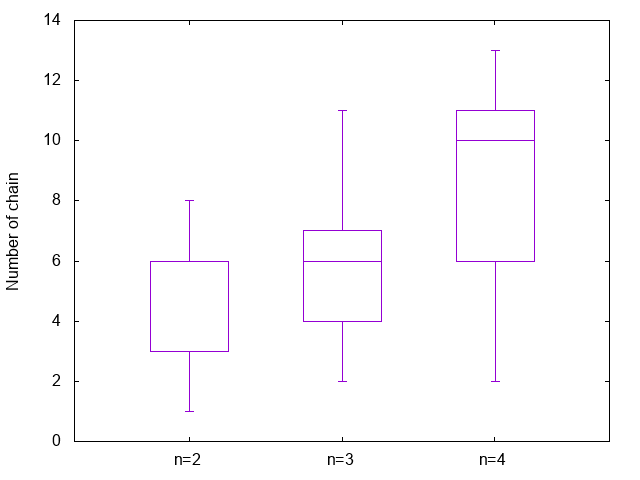
\includegraphics[height=7cm]{experiment/Potential/KAI/graph/chain_N2_4.png}
  \caption{ポテンシャル最大化法の探索深度nの変更による連鎖数への影響;なおn=2の時の中央値は3} \label{fig:poten_chain_depth}
\end{center}
\end{figure}


\begin{table}[tb]
\begin{center}
\caption{ポテンシャル最大化法の探索深度nの変更による影響)} \label{tab:poten_depth}
\begin{tabular}{|l|c|c|c|} \hline
探索深度n & 平均連鎖数 & 平均スコア & 1手あたりの平均計算時間[ms]\\ \hline
2 & 4.04 & 8071.0 & 1.16\\ \hline
3 & 5.96 & 18883.2 & 11.75\\ \hline
4 & 8.36 & 45925.6 & 1249.98\\ \hline
\end{tabular}
\end{center}
\end{table}

\section{全幅探索}
\subsection{変更の内容}
探索の深さを$n=3$から$n=4$へと増加させることで、連鎖効率が大きく増加することが分かった。しかし、それが探索深さによるものか、探索幅によるものかを検証したい。ぷよぷよでは3手目以降が分からないため、探索幅であるツモの種類を限定することは難しい。そこで、深さを減らした状態で全幅探索を行い、その変化を調べる。具体的には、探索深さを$n=3$としたとき、3手目のツモを予告ぷよに限らず全て列挙し、探索に利用する。

探索量の増加が予想されるが、今回は探索するツモの種類が増えるだけであり、通常のポテンシャル最大化法に対し高々10倍である。本来のポテンシャル最大化法に必要な計算時間は0.01秒程度であり、それが10倍に増加することは無視できる範疇に収まる。

確定しているはずのツモを全幅探索とすることで、盤面予測の精度が下がり、連鎖効率が低下する可能性も懸念される。他方、単純に探索量の増加が連鎖数の向上に役立つ可能性もある。連鎖数がどのような分布になるか、前述の$n=3$、$n=4$の時と比較を行った。

\subsection{結果と考察}
シミュレーションの結果により得られた連鎖数の分布を図\ref{fig:poten_chain_width}に、その時の平均連鎖数、平均スコア、1手当たりの平均計算時間を表\ref{tab:poten_width}に示す。平均連鎖数は単純な$n=3$の時よりも0.74増加し、また$n=4$には及ばなかった。このことから、$n=4$としたときの連鎖数の上昇は、探索の深さによる影響と幅による影響の両方があることが分かる。

全幅探索は3手目のツモに対して行っているため、本来は不要な処理である。また、手の選択には最大化戦略のみを用いているため、都合の悪いツモはすべて無視され、都合の良いツモのみが考えらえることになる。よって、本来の盤面状況とは乖離した予測が行われ、連鎖数が低下する可能性すらあった。それが改善された理由は、人間の連鎖構築手法を考えてみると理解がしやすい。人はぷよをフィールドに置くとき、現れてほしい色を想像しながら意思決定を行っている。赤色を消そうとしたときに、青色で代用することはできない。しかし従来の連鎖ポテンシャル法では、理想的な配色が来なかった場合に、無理やり別の色を使う道筋を立てて連鎖構築を行う。そこには代用できないものを代用しようとする無理があり、全幅探索ではそれを改善することが可能といえる。例え実際には来ていないツモでも、その可能性を視野に入れることで、最適な方策を取れたと考えられる。

ただし、適するツモが来なかった場合の連鎖数は一段と低く、最終的にどのツモでもぷよを消せない結果も現れた。それでも、箱ひげ図の箱は$n=3$より全体的に上に位置することから、多くの場合で全幅探索による連鎖数の向上の影響が見られたといえる。

また計算時間は約0.04秒と、リアルタイム性になんら問題ない値であった。この結果から、全幅探索は実用レベルのアルゴリズム改善策であることが示された。しかし、25%が5連鎖から0連鎖の範囲にあり、無視できない回数が非効率な連鎖となってしまっている。高い連鎖数をより安定させるための改善が、さらに必要である。

\begin{figure}[tb]
  \begin{center}
  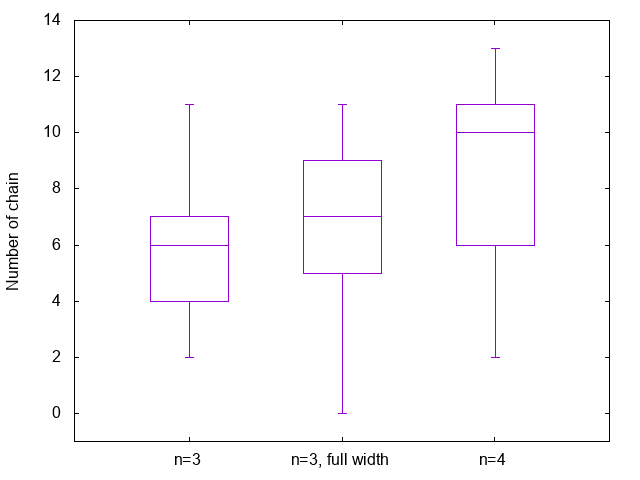
\includegraphics[height=7cm]{experiment/Potential/KAI/graph/chain_full.png}
  \caption{ポテンシャル最大化法の全幅探索による連鎖数への影響} \label{fig:poten_chain_width}
\end{center}
\end{figure}


\begin{table}[tb]
\begin{center}
\caption{ポテンシャル最大化法の全幅探索におけるシミュレーション結果)} \label{tab:poten_width}
\begin{tabular}{|c|c|c|} \hline
 平均連鎖数 & 平均スコア & 1手あたり平均計算時間[ms]\\ \hline
6.68 & 29220.2 & 41.59\\ \hline
\end{tabular}
\end{center}
\end{table}


\section{消去する手の有効化}
\subsection{変更する内容}
従来の連鎖ポテンシャル法では、1手目にぷよを消去する手を必ず除外してきた。しかし、人が実際に連鎖構築を行う際には、無駄なぷよを消して整地するなどの行為が行われる。必要最低限の消去を許すことは、AIの連鎖構築においても有効であると考えられる。

そこで、1手目に消去する手を除外せずに連鎖構築を行うアルゴリズムについて、実装しシミュレーションを行った。着手の評価値は、1手目で消去した点数を無視し、2手目以降で発火する連鎖のスコア値にしている。これは、消去する行為が評価値に加算され、毎回細かくぷよの消去を行う状態に陥ることを防ぐためである。

探索精度が悪い状態で消去する手を許可すれば、無意味な消去が生じることで、同じ手での構築連鎖数が下がることになる。それはすなわち、ツモを効率的に活かして連鎖を構築できていないことを意味する。他方で、消去により無駄なぷよを的確に処理し、長期的に連鎖数を向上させられることが、理想的な期待される成果である。消去しない方法であった通常のポテンシャル最大化法、全幅探索を行う手法の2種類について、連鎖数を比較し検討を行った。

なお、この手法による探索時間の増加は、わずかなものにとどまると考えられる。考慮していなかった数手分が計算に加わる程度であり、計算量のオーダは変わらないためである。

\subsection{結果と考察}
1手目で消去することを許可したアルゴリズムの連鎖数について、分布を比較したグラフを図\ref{fig:poten_chain_del}に示す。またこのときの平均連鎖数、平均スコア、1手当たりの平均計算時間を表\ref{tab:poten_del}に示す。

通常のポテンシャル最大化法に対し消去を許可することでは、大きな改善は見られなかった。平均連鎖数は5.96から5.86へとわずかに減少したことから、この方法は妥当ではないと結論付けた。

一方、全幅探索に消去の許可を与えた場合には、大きな改善が見られた。$n=4$のときの平均連鎖数8.36には及ばないものの、8連鎖近くになる平均連鎖数と、構築連鎖数の安定が確認できた。最低連鎖は外れ値として0連鎖や1連鎖が存在するものの、最大連鎖は$n=3$ではこれまで無かった13連鎖が確認できた。構築された連鎖の75%は7連鎖以上であり、残りの25%もおおよそ7連鎖から4連鎖の範疇に収まる。これは通常の連鎖ポテンシャル法よりも、全体的に連鎖数の分布が向上していることを意味している。

この結果の理由を理解するために、図\ref{fig:poten_totalPuyo_del}にフィールド上のぷよ数の推移を示した。数値は、横軸が手数であり、縦軸は発火直前に設置されているぷよの数の平均である。

消去を許可しない場合には、消せずには置けない場合を除外してやり直しているため、必ず33手目でぷよが66個に達し、発火となる。一方、単純に消去を許可すると、ごく序盤の5手目付近からフィールドのぷよ数が少なくなり、最終的に平均20個近くのぷよを消去していることが分かる。つまり、評価が適切に行われていないために無駄な消去が生じ、ぷよが少なくなることで連鎖数にも影響を及ぼしたと考えられる。

他方、全幅探索を行った場合にはほとんど消去が行われていない。フィールドがほぼ完全に埋まる終盤になってから通常の手法との差が見られ、大きく減少するのは最後の手のみである。おそらく、フィールドが埋まったことで連鎖を伸ばす余地が無くなり、必要に駆られて消去を行い始めているものと思われる。逆に考えると、不必要な消去は行われておらず、ツモを有効に利用して連鎖を構築している。

探索の幅がさらに増加したことで、全幅探索、消去ありの場合の計算時間は増加している。それでも0.05秒であり、リアルタイム性に何ら問題ないものと考えられる。総じて、連鎖ポテンシャル法を改良する方法として全幅探索、1手目の消去を試行したが、この両方を用いることが連鎖数の向上に有効であると確認できた。この手法では、構築連鎖数の向上が見られ、さらにリアルタイム性と連鎖の柔軟性を維持している。連鎖構築アルゴリズムの改善策として、有効であったと結論付けられる。


\begin{figure}[tb]
  \begin{center}
  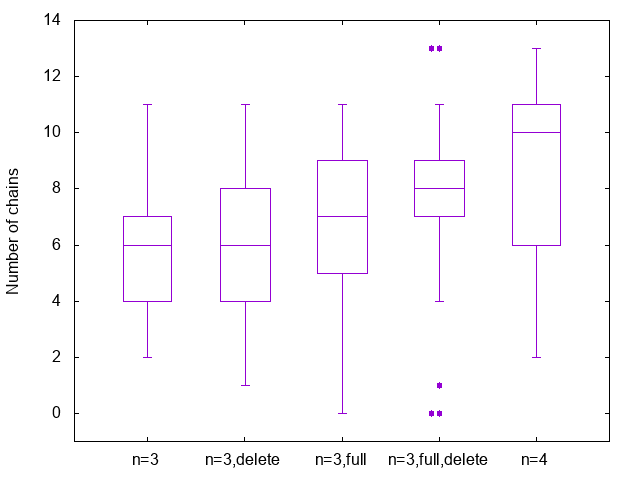
\includegraphics[height=7cm]{experiment/Potential/KAI/graph/chain_del.png}
  \caption{ポテンシャル最大化法の消去許可時における連鎖数への影響} \label{fig:poten_chain_del}
\end{center}
\end{figure}


\begin{table}[tb]
\begin{center}
\caption{ポテンシャル最大化法の消去許可時におけるシミュレーション結果)} \label{tab:poten_del}
  \begin{tabular}{|l|c|c|c|} \hline
アルゴリズム & 平均連鎖数 & 平均スコア & 平均計算時間[ms]\\ \hline
$n$=3、1手目消去あり & 5.86 & 17959.8 & 14.42\\ \hline
$n$=3、全幅探索、1手目消去あり & 7.78 & 37379.8 & 53.82\\ \hline
\end{tabular}
\end{center}
\end{table}


\begin{figure}[tb]
  \begin{center}
  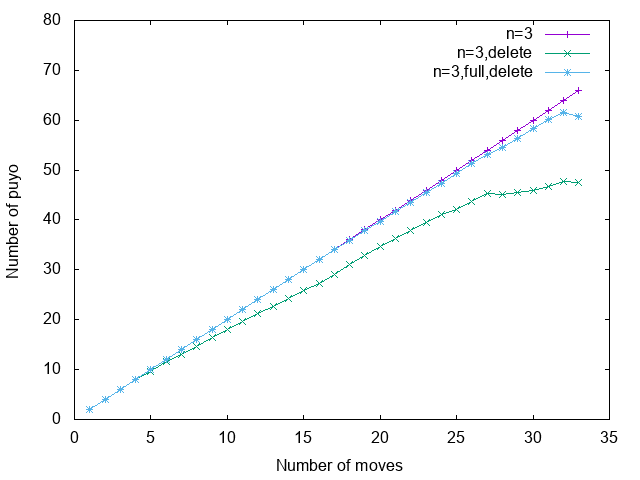
\includegraphics[height=8cm]{experiment/Potential/KAI/graph/totalPuyo_N3_N3del_N3fulldel.png}
  \caption{連鎖ポテンシャル法の消去許可時におけるフィールドのぷよ数推移} \label{fig:poten_totalPuyo_del}
\end{center}
\end{figure}


%\section{ツモ選択と置き方選択の区別}

\section{全体を通しての考察}
ここまで、連鎖ポテンシャル法の改善手法について検討してきた。結果として、探索深度を増加させること、1手目の消去を許可したうえで全幅探索を行うこと(以下、「改善法」とよぶ)、によって構築連鎖数を約2連鎖改善できることが分かった。

この改善が、どのような影響によるものか考察するために、図\ref{fig:poten_tsumoList}を用意した。これは、各手の探索において最大の評価値を得られた手数の数を表している。すなわち、探索によって得られた候補手の数である。候補手が少ないときにはツモを置ける場所は限られており、逆に候補手が多い時にはフィールドの受けが広いことを示す。分かりやすさのために、通常のポテンシャル法、改善法、探索深度$n$を4とした時の3手法について載せた。横軸は手数である。

3手法においてほとんど同じであるのは、1手目から3手目までの最序盤、および26手目以降の終盤である。また、16手目から25手目の中盤では、$n=4$とした手法が候補手の数は少なく、$n=3$と改善法がほぼ同等の水準にある。そして、4手目から14手目の序盤では、通常の手法、改善法、$n=4$の順に候補手が多い。この順は、そのまま構築連鎖数の大きさの順である。そこで構築された連鎖数の違いは、この序盤の候補手数の差によって現れたのではないかと考えられる。

\begin{figure}[tb]
  \begin{center}
  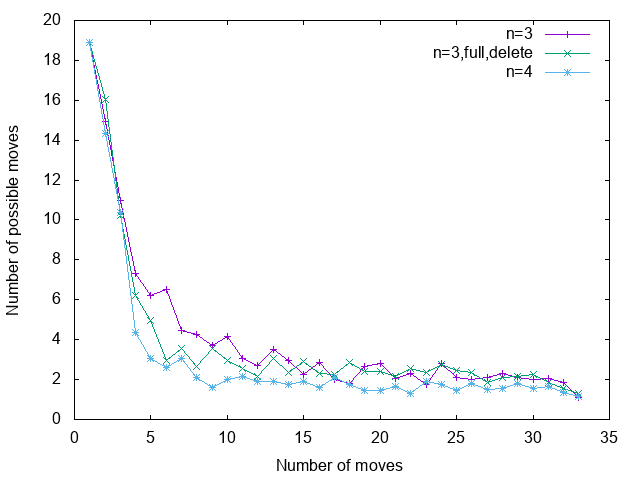
\includegraphics[height=9cm]{experiment/Potential/KAI/graph/tsumoList_D3_fulldel_D4.png}
  \caption{ポテンシャル最大化法の改良手法における候補手の数の推移} \label{fig:poten_tsumoList}
\end{center}
\end{figure}

候補手が絞り込めていない状態は、ツモを配置できる場所が多い、受けの広い形と捉えることもできる。しかしポテンシャル法に関しては、それが連鎖数に悪い影響を与えることが考えられる。探索により、最適な手を特定できていないといえるためである。反対に候補手を絞ることで、効率の良い連鎖形への道筋が立てられ、それに沿うような連鎖構築が可能になる。全幅探索による連鎖数の改善は、そのような理由によるものであった。そして、それは特に序盤の手に関して、強い影響が存在する可能性が浮上した。通常の手法と改善法では最終的な連鎖数に2近くの差があり、候補手の数の差は序盤に現れていた。

中盤以降で候補手の数は大きく変わらないことを考えると、序盤で構築された連鎖の形によって、その後の連鎖数の伸びが変わるといえる。すなわち、序盤でどのような手を選択してツモを配置するかが、重要といえる。序盤ではフィールド上のぷよの数はそう多くないため、比較的候補手の数も多い事がグラフから読み取れる。これをいかに絞り、序盤の連鎖を構築するかが、ポテンシャル最大化法の改善の鍵を握っていると思われる。


\section{対「のほほ」戦}
最後に、改善された連鎖ポテンシャル法を用いて、ゲーム内AIとの対戦を行った。対戦相手はDQNでも対象とした「のほほ」にし、DQNの学習によって得られたAIとの比較を行えるようにした。よって、ゲームソフトと設定は同様のものを使用した。

なお、実験にあたっての環境はRLEで用いているものと同様のエミュレータ(snes9x)とし、インターフェイスは盤面状態の入力を画像認識で、ぷよの設置出力をキーボード操作で、それぞれ実装した。連鎖ポテンシャル法は連鎖を構築するだけのアルゴリズムであるから、連鎖を発火するためには別の方針が必要となる。ここでは、現在のツモで閾値を超えたスコアの連鎖を発火できる場合、即座に発火することとした。閾値はDQNで行われた試合のスコア(表\ref{tab:dqn_score_vs})を参考として、2100点(4連鎖相当、5段分のおじゃまぷよ)と余裕を持たせた4200点(5連鎖相当、10段分のおじゃまぷよ)の2種類について実行した。

対戦の結果は、表\ref{tab:poten_vs}に示す。DQNによるAIと比べ、明らかにスコア、勝ち数で上回った。スコアでは「のほほ」を圧倒し、連鎖構築能力の高さが示された。特に、閾値を2100とした時の方が双方のスコアが高かった。2100点は画面全てが埋まりきらない量のおじゃまぷよを送るために1回の連鎖では埋めきれなかったり、ちょうどよく「のほほ」との相殺が起きるような点であったりしたことによるものと考えられる。一方で4200点では、発火できれば相手を埋められることで勝負が決まるため、「のほほ」の点数が低い。改良法側のスコアも低いのは、連鎖構築と発火により多くの手数がかかり、発火率が低いためであると思われる。

一方で、勝敗は5分か負けであり、「のほほ」の強さが示された。「のほほ」はぷよを3段目に積まずに、その横に高く積む。そのため、おじゃまぷよで埋めて倒すには12段分のおじゃまぷよが必要であること、おじゃまが降った後でもその横にあるぷよを問題なく消せること、などが強さに影響した。改善法では3段目も使って連鎖を構築するので、おじゃまが降れば「のほほ」よりも少ない段数で埋められてしまい、それが負けにつながった。

それでも、対戦でおじゃまぷよによる妨害がある中、連鎖を構築し、ゲーム内のAIと連鎖合戦を行い勝負を競えるレベルにあった。今回は考慮していない、対戦の戦術面に関して強化を施すことで、より強いAIを実現できるものと期待される。

\begin{table}[tb]
\begin{center}
\caption{ポテンシャル最大化法の改善法を用いた「のほほ」との対戦結果} \label{tab:poten_vs}
  \begin{tabular}{|l|c|c|c|} \hline
スコア閾値 & 勝敗 & 改善法の & 「のほほ」の\\
 & (改善法--のほほ)& 平均スコア & 平均スコア\\ \hline
2100 & 25--25 & 4983.62 & 2863.90\\ \hline
4200 & 21--29 & 4047.12 & 1656.44\\ \hline
\end{tabular}
\end{center}
\end{table}


\chapter{人間の知識を適用したAIの作成} \label{human} \setcounter{section}{0}
ポテンシャル法の改良手法では、全幅探索と1手目の消去の許可が有効であった。この改良法によって連鎖数が伸びた原因として、序盤から候補手を限り、より良い連鎖を構築していた可能性があった。この手法をさらに改良するためには、さらなる序盤の効率化が考えられる。この可能性を検討するため、人の連鎖構築知識を基にしたAIを作成し、その組み合わせを行った時の連鎖構築について評価を行う。

\section{連鎖構築知識の抽出と実装}
ぷよぷよのプレイヤーは、練習次第で13連鎖をも超える連鎖を構築することができる。その連鎖構築知識をAIに活用することで、その性能を向上させることができると考えるのは自然である。

一方、ぷよぷよの盤面は78マスに4色の色が設置されることから、膨大な状態の組み合わせが存在する。これを単純にルール化することは難しく、何らかの工夫が必要である。ただし今回は、ごく序盤の手数のみを対象とすることから、あまり多くの状態にはならないと思われる。そこで連鎖形を、もっとも基本的な形である3--1階段5連鎖(図\ref{fig:teikei},\ref{fig:kaidan5}参照)に絞り、そこへ至る着手をif--thenルールで記述した。

if--thenルールは筆者の手で記述し実装した。そのルールを単純化して以下に示す。実装の際には、設置法を記述するため、左右や上下の入れ替えなどで条件分岐がより増える。なお、便宜的に色をABCなどの記号化している。例えば、現在のツモが「赤青」で、次のツモが「緑青」ならば、「ABBC」と記号化できる。また「ゾロ」はツモの2つのぷよが同色であることを示し、3-1階段のうち3つの縦部分を「土台」、隣の列に置く1つのぷよを「仕掛け」とする。

\begin{lstlisting}[basicstyle=\ttfamily\footnotesize, frame=single]
ツモがゾロである:
    土台が1つでツモが同色の列が存在 or
    土台が0個で、隣列に同色の土台がない列が存在:
        その列に縦置き
    土台が3つ以下でツモが同色の列が存在し、かつ
    右隣の列の土台が3つ以上で仕掛けが無い:
        その列と右隣の列に横置き
    その他:
        左端の列に立てて置く
ツモがゾロでない:
    ツモの一つと同色の土台が存在する:
        ツモと同色の土台が隣り合って存在し、かつ
        両土台が3つ以下:
            色が揃うように横置き
        左端列の土台が2つでツモに土台の色が含まれる:
            左端列に縦置き
        ツモと同色の土台が隣り合って存在し、かつ
        右列の土台が2つ:
            土台と仕掛けを完成させる縦置き
        ツモの1つと同色の土台が存在し、かつ
        その右の列の土台が3つ以上であって仕掛けが無い:
            さらにその右の列の土台が(ツモの1つと同色or空):
                仕掛けの列とその右の列に横置き
            その他:
                仕掛けの列に縦置き
        ツモの1つと同色の土台が存在し、その右列が空列:
            土台を1つ増やす横置き
    その他:
        隣り合う2列が空列:
            その左の列の土台にツモの色が含まれる:
                左の土台と繋げないように、空列に横置き
            ツモがABBBである or
            ツモがABACである or
            ツモがABCCBBである:
                空列に対し左がB、右がAとなるよう横置き
            その他:
                空列に対し左がA、右がBとなるよう横置き
        その他:
            左端の列に縦置き
\end{lstlisting}

主な手順としては、左から優先して同じ色を縦に並べ、3つのつながりを作った後、隣の列に仕掛けとなる4つ目のぷよを置く流れである。非効率な部分(適するツモが無い場合、左端に捨てるなど)があるものの、ルールベースによるAIを完成させた。あまり細かいルールとしていないのは、ポテンシャル最大化法と組み合わせる際の、序盤の手順としてのみ用いることを想定したためである。

この手法を用いて序盤数手分を設置したのち、改良法による連鎖構築によるシミュレーションでどれほど連鎖構築能力が向上するかを確かめた。なお、シミュレーションの環境はポテンシャル最大化法の時と同様で、ツモも同一のものを用いた。また、手数は図\ref{fig:poten_tsumoList}を参考にし、4手から14手まで2手ずつ変化させてそれぞれの構築連鎖数を調べた。さらに、「のほほ」との対戦に用いた2100点という閾値を参考にし、任意のツモで2100点以上の連鎖を発火できるようになるまでの手数を調べた。


\section{結果と考察}
人の知識を用いた手法を利用した手数と、シミュレーションによる連鎖数との関係を図\ref{fig:human_chain}に示す。全体的に同じような分布であり、大きな差は無いといえる。また、最終的な連鎖数の平均と、スコア2100点に達するまでの平均手数を、表\ref{tab:human}に示す。わずかな違いであるが、人間の知識による着手を6手分用いたときの平均連鎖数がもっとも高い。この差は、低い連鎖が減ったことで平均が底上げされたことによると考えられる(図\ref{fig:chain_poten_human}参照)。同時に、外れ値が出ずに連鎖数の分散が小さくなったことが示された。人の知識を適切に用いることで、連鎖を安定させることができることが示された。それ以外の結果では悪化しており、連鎖数の向上に役立たないことがわかった。

2100点までの到達手数においても、人間の知識を用いた中で6手分の時がもっとも低い値であるが、人間の知識を用いない場合の方が低かった。これは、6手以外では序盤の連鎖を組む効率が低下したことを意味している。人の知識を6手分用いた場合では、大きな低下にはなっていないものの、序盤の連鎖構築に関して有効な改善法では無かった。

図\ref{fig:human_tsumoList}に、ポテンシャル最大化法の改善法と、探索深さを4にした手法、人の知識を利用した手法における候補手の推移を示す。人の知識を用いた方法では、6手までルールによって候補手がただ一通りに決まっている。7手目からはポテンシャル最大化法の改善法に切り替わり、10手目までは比較的候補手が絞られている。しかし、その後は人の知識を使わない場合と同等以上の数値であり、改善されていない様子が見られる。他方で、このような複数の手を打てる状態が連鎖の柔軟性を増し、連鎖数の安定に寄与したと捉えることもできる。人の知識により最序盤に連鎖形を土台として固めることで、その後多くの状態に対応できる連鎖を構築できたと考えられる。

この手法をさらに改善するために検討すべき要素として、階段5連鎖を用いたこと、if--thenルールの問題、ポテンシャル最大化法との相性、そもそも序盤の影響はそう大きくない、などが考えられる。序盤の手を階段5連鎖に絞ることで、ツモを活かせない場面や、その連鎖構築の流れをポテンシャル最大化法が有効に利用できない場面などが生じうることから、他の連鎖形や、あるいは連鎖になっていない序盤の置き手順などをさらに検討する必要がある。序盤の連鎖効率は、if--thenルールを変更することでさらに改良できると思われるため、ここにも改善の余地が残る。人の連鎖構成法と、AIによる連鎖構成法はそもそも違うため、その2つをつなげる工夫が必要であるかもしれない。このような検証をさらに重ね、連鎖構築AIの改良とその影響をさらに調べることは、今後の課題である。

\begin{figure}[tbp]
  \begin{center}
  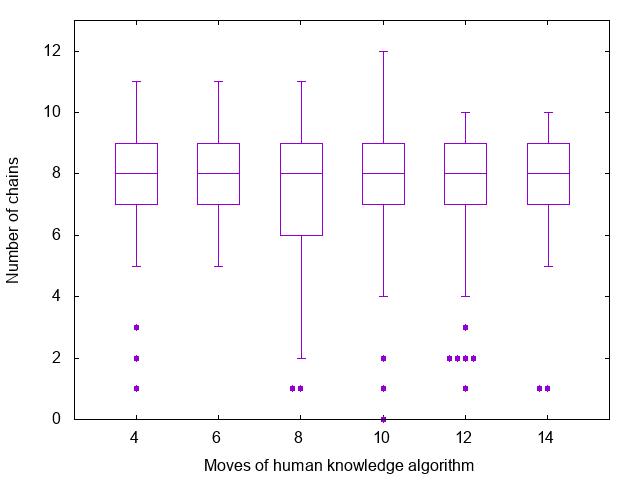
\includegraphics[height=7cm]{experiment/HumanKnowledge/human_chain.png}
  \caption{人の知識を用いた連鎖構築法の利用手数と連鎖数} \label{fig:human_chain}
\end{center}
\end{figure}


\begin{figure}[tbp]
  \begin{center}
  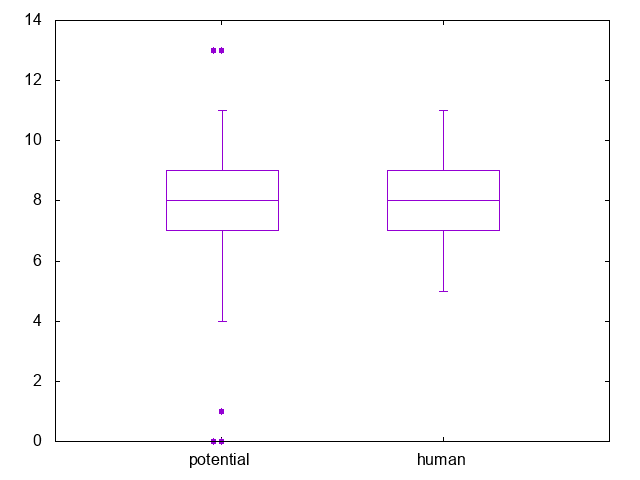
\includegraphics[height=7cm]{experiment/HumanKnowledge/chain_poten_human.png}
  \caption{ポテンシャル法の改良手法と人の知識を用いた連鎖構築法の比較} \label{fig:chain_poten_human}
\end{center}
\end{figure}


\begin{table}[tbp]
\begin{center}
\caption{人の知識を用いた連鎖構築法の利用手数と連鎖構築} \label{tab:human}
  \begin{tabular}{|r|c|c|} \hline
人の知識を用いた手数 & 33手目平均連鎖数 & 2100点までの平均手数\\ \hline
なし& 7.78 & 14.78\\ \hline
 4 & 7.72 & 15.54\\ \hline
 6 & 8.10 & 15.16\\ \hline
 8 & 7.46 & 16.04\\ \hline
10 & 7.78 & 17.64\\ \hline
12 & 7.34 & 18.66\\ \hline
14 & 7.56 & 20.60\\ \hline
\end{tabular}
\end{center}
\end{table}


\begin{figure}[tbp]
  \begin{center}
  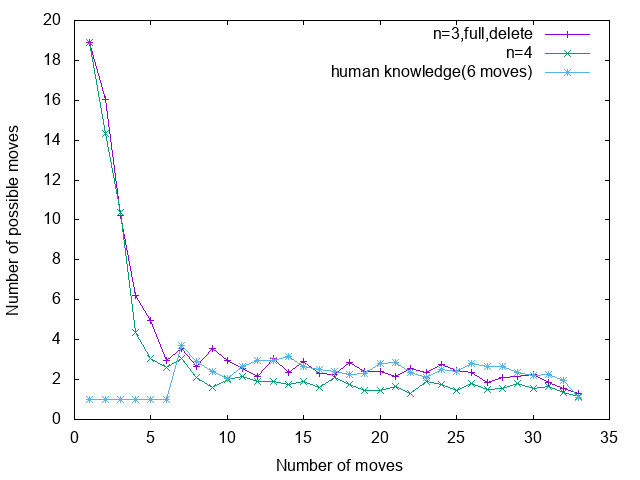
\includegraphics[height=9cm]{experiment/HumanKnowledge/human_tsumoList.png}
  \caption{人の知識を利用した手法における候補手の数の推移} \label{fig:human_tsumoList}
\end{center}
\end{figure}


\section{対「のほほ」戦}
ポテンシャル最大化法と同様に、ゲーム内AIである「のほほ」との対戦を行い、その成績を評価した。連鎖発火の閾値は2100とし、人の知識を用いるのは6手とした。その他の条件は、ポテンシャル最大化法で対戦を行った時と同等である。

対戦の結果は、表\ref{tab:human_vs}に示す。おおよそ対等な勝敗であり、またスコアが「のほほ」に比べて高いことも、ポテンシャル最大化法での対戦結果(表\ref{tab:poten_vs})と同じであった。若干のスコアの低下があるのは、ほとんど誤差であるといえるだろう。ただし、発火手数が遅れたことによる影響の可能性は排除できない。常に高速でぷよを落下させる「のほほ」の連鎖に対抗するには、素早く連鎖を放つことが必要であった。

また、当然ながら6手目までは階段連鎖を構築しようとする動きを見せた。ポテンシャル最大化法に切り替わった後、その連鎖の流れに沿って連鎖を伸ばすこともあれば、完全に無視してぷよを設置する場面もあった。このような動きからは、人の知識をAIに応用するにも、単なる置き方のみに留まらず、その理屈や目指す形などを適用することも有効である可能性がある。一方で、序盤の設置法といった部分的な知識を与えるだけでも、AIの行動にある程度の方向性をつけられることもあり得る。人を手本としたAIはそのような点で、さらなる工夫の余地と可能性が残っているといえる。


\begin{table}[tbp]
\begin{center}
\caption{人の知識を利用した手法による「のほほ」との対戦結果} \label{tab:human_vs}
  \begin{tabular}{|l|c|c|} \hline
勝敗(実装AI--のほほ) & 実装AIの平均スコア & 「のほほ」の平均スコア\\ \hline
 24--26 & 4762.52 & 2703.74\\ \hline
\end{tabular}
\end{center}
\end{table}


\chapter{結論} \label{ketu} \setcounter{section}{0}
\section{研究成果}
本研究では、不完全情報ゲームの一種である「ぷよぷよ」によるAI構築を通して、ディープラーニングとQ学習を組み合わせたDQNを用いたゲームAIと、人の知識を基にしたルールベースのゲームAIの比較を行った。DQNを用いた場合には高々5連鎖を構築することが精一杯であり、それも安定したものではなかった。一方で人の知識を基にしたAIでは、32手での連鎖構築シミュレーションにおいて、平均8.1の連鎖を構築することができた。この時、最低連鎖は5連鎖、最大連鎖は11連鎖であり、DQNに比べると安定して大連鎖を構築できていた。

また、これらAIの強さを比較するために、ゲーム内AIとの対戦を行った。50戦行った結果、DQNによるAIでは2--48、人の知識を用いたAIでは24--26となり、人の知識によるAIが圧倒的な強さであった。人の知識を利用したAIでは、対戦の平均スコアでゲーム内AIを大きく上回っており、その連鎖構築能力の高さが示された。対戦のための戦術に関する知識を加えたAIを実装することで、十分にゲーム内AIを上回る強さを発揮できると予想される。

今回はぷよぷよの対戦AIの強さとして特に連鎖構築能力を取り上げ、その連鎖威力、リアルタイム性、柔軟性を維持、向上させることを目指した。DQN、人の知識の適用の双方でその目的を達するための学習ができたが、その強さには大きな違いが現れた。その差は連鎖威力の差であり、効率的で安定的な連鎖を構築するための手法を確立することが、ぷよぷよの強いAIにとって重要な点であった。そのためには人の知識を基にしてAIを設計、学習することが有効であると考えられる。

今回のAIは平均連鎖が8連鎖程度であったが、ある程度練習を積んだぷよぷよプレイヤーであれば、安定的に10連鎖以上を構築することも難しくはない。そのような状況において、ぷよぷよAIの強さは未だ不十分であるといえる。これをさらに改善するためには、人の知識をいかにしてAIに取り入れるかを、より検討してゆくことが求められる。


\section{今後の課題}
DQNを始めとする、ニューラルネットを用いたAIは学習が自動で行える利点があるものの、中身がブラックボックスであることが欠点である。改善を行おうとしても、どのように学習が行われ、何が問題であるかが非常にわかりづらい。多くの学習時間を費やして、トライアル&エラーを行うしかないのが現状である。

一方で、人の知識をAIに用いることは、その膨大な知識の抽出とルール化・実装に関して多大な手間がかかる。すべての知識を余すことなく記述できるかどうか、不必要な知識が紛れていないかなど、必ずしも明確なルールが確立できない問題もある。知識を体系化した上で、どのように実装すると有効であるかを確かめることもまた、大きな課題として残っている。

そこで次の段階として、ニューラルネットによる曖昧な部分と、人の知識による厳密なルールとを、組み合わせて使うことを課題とする。それぞれが補間しあうような関係となり、人の断片的な知識を基に学習が行われ、より最適化されたルールが構築されることが理想として考えられる。必要最低限の知識を用いた学習により、より効率的で有効なAIが実現できる可能性がある。そのような手法の確立を行い、より人を楽しませるAIを構成することが、今後の課題である。

\clearpage
%参考文献
\addcontentsline{toc}{chapter}{参考文献}
\bibliographystyle{jplain}
\bibliography{ref}

\section*{謝辞}
当研究において、ご指導いただき、また多くのご迷惑をおかけした主任指導教員の橋山智訓先生には格別の感謝とお詫びを申し上げます。また、日頃より愉快なお話で皆を盛り上げてくださる副指導教員の田野俊一先生、影ながら支えてくださる事務の岸本雅代さんにも御礼申し上げます。研究室の学生の皆さんにも、研究に役立つ刺激を大いにいただき、励まされています。皆さんの暖かなご支援に感謝いたしたく、謝辞とかえさせていただきます。


\end{document}

